\documentclass{homework}
\usepackage[dvipsnames]{xcolor}
\usepackage{hyperref}
\usepackage{csquotes}
\hypersetup{
    colorlinks=true,
    linkcolor=blue,
    filecolor=blue,      
    urlcolor=blue,
}
\usepackage[utf8]{inputenc}
\usepackage[english]{babel}

\usepackage[
backend=biber,
style=bwl-FU,
sorting=ynt
]{biblatex}

\addbibresource{sample.bib}
\usepackage{listings}
\usepackage{graphicx}
\graphicspath{ {./images/} }
\usepackage{float}
\usepackage[ruled,vlined]{algorithm2e}

\title{Statistical Learning Theory Homework}
\author{Quentin Le Roux}

\begin{document}

\maketitle

\exercise[-- Part 1: Preliminaries]

We consider the $d$-dimensional observations $x_1, ..., x_n$, associated to responses $y_1,...,y_n\in\mathbb{R}$.

\subsection*{I.1}
Given $\mathcal{H}$ a hypothesis space of function $h$ such that $h:\mathcal{X} \rightarrow \mathcal{Y}$ with $\mathcal{X}$, the input space, 
and $\mathcal{Y}$, the output space, we recall the definition:
$$\mathcal{H} = \{h:x\rightarrow w^Tx \quad{s.t.}\quad w\in\mathbb{R}^{d}\}$$ 
Given:
\begin{itemize}
    \item $\forall i \in \{1, ..., n\},\,\, (x_i, y_i) \in \mathbb{R}^d \times \mathbb{R}$, the centered data points
\end{itemize}
In the case of a linear regression, non-centered data helps model a scalar product $Y$ (the target) as a 
function of the data's input vector $x$ such that:
$$y=w^Tx+b$$ 
Given:
\begin{itemize}
    \item b,  the intercept
\end{itemize}
Notationally, we can use a homogeneous coordinate representation where 1 is appended or pre-pended 
to the feature vector $x$ such that, for instance:
$$x_{non-centered}=x_{nc}=(1\quad x^T)^T \in \mathbb{R}^{d+1}\quad{s.t.}\quad x_{nc}=(1, x_1, ..., x_d)^T$$
$$w_{non-centered}=w_{nc}=(b\quad w^T)^T \in \mathbb{R}^{d+1}\quad{s.t.}\quad w_{nc}=(b, w_1, ..., w_d)^T$$

As such, we can modify our previous representation of the hypothesis space $\mathcal{H}$ 
such that for non-centered data we obtain $y=w_{nc}^T.x_{nc}$.

We conclude that: 

\textcolor{OliveGreen}{$$\mathcal{H} = \{h:x_{nc}\rightarrow w_{nc}^Tx_{nc} \quad{s.t.}\quad w_{nc}\in\mathbb{R}^{d+1}\}$$}

\subsection*{I.2}
For the sake of brevity, we will denote $w_{non-centered}$/$w_{nc}$ as $w$, and $x_{non-centered}$/$x_{nc}$ as $x$.

We recall the definition of a scalar product $\langle a, b\rangle$ given $a, b \in \mathcal{R}^{d+1}$ (indexed at 0):
$$\langle a, b\rangle = \overset{d}{\underset{j=0}{\sum}}a_j.b_j$$
We also recall the target vector $\hat{y}$ such that $y=w^Tx$. As such, if we denote as $\hat{y}_i$ the associated predicted value for the
observation $x_i$, we can write the following expression:
$$\hat{y}_i=w^Tx_i=b+\underset{j=1}{\overset{d}{\sum}}w_j.x_{i, j}$$
If we  denote the first element of $x_i$ as $x_{i, 0}$ equal to $1$, and the first element of $w$ as $w_0$ equal to $b$, we can
rewrite the formula above such that:
$$\forall i \in \{1, ..., n\},\,\, x_i=(x_{i, 0}, x_{i, 1}, ..., x_{i, d})^T\in\mathbb{R}^{d+1}\quad{with}\quad x_{i, 0}=1$$
$$\forall i \in \{1, ..., n\},\,\, w_i=(w_{i, 0}, w_{i, 1}, ..., w_{i, d})^T\in\mathbb{R}^{d+1}\quad{with}\quad w_{i, 0}=b$$
$$\hat{y}_i=w^Tx_i=\underset{j=0}{\overset{d}{\sum}}w_j.x_{i, j}$$
We conclude that:

\textcolor{OliveGreen}{We can rewrite $\hat{y}_i$ by using the definition of the scalar product such that:
$$\forall i\in\{1, ..., n\}\quad \hat{y}_i=\langle w, x_i\rangle$$}

\subsection*{I.3}

Given the results obtained in \textbf{I.1} and \textbf{I.2}, we can express the hypothesis space for non-centered data as:
$$\mathcal{H}=\{h:x\rightarrow\langle w, x\rangle \quad{s.t.}\quad w\in \mathbb{R}^{d+1}\}$$ 
Given:
\begin{itemize}
    \item $\forall i \in \{1, ..., n\},\,\, (x_i, y_i)$, the non-centered datapoints
    \item $\hat{y}_i=h(x_i)$, the associated predicted values
\end{itemize}

We then define the squared loss function $l$ such that:
$$l(y_i, \hat{y}_i)=(\hat{y}_i - y)^2 = (h(x_i) - y)^2=(w^Tx_i-y_i)^2$$

We conclude that:

\textcolor{OliveGreen}{We can define $R$, the empirical risk associated to $h$ with $l$ the squared loss function, such that:
$$R(h)=\frac{1}{n}\underset{i=1}{\overset{n}{\sum}}l(y_i, h(x_i))=\frac{1}{n}\underset{i=1}{\overset{n}{\sum}}(h(x_i)-y_i)^2=\frac{1}{n}\underset{i=1}{\overset{n}{\sum}}(w^Tx_i-y_i)^2$$}

\subsection*{I.4}

Given the objective function $R$ previously stated in \textbf{I.3}, we may penalize it by adding the euclidean norm of $w$, denoted
$||w||^2$, multiplied by a strictly positive regularization parameter $\lambda$. As such, we can write:

\textcolor{OliveGreen}{$$F(w)=R_{penalized}(h)=\frac{1}{n}\underset{i=1}{\overset{n}{\sum}}(w^Tx_i-y_i)^2+\lambda||w||^2$$
Given:
\begin{itemize}
    \item $||u||^2=\underset{j=0}{\overset{d}{\sum}}u_j^2$
    \item $\lambda > 0$
\end{itemize}}

\subsection*{I.5}

Given the newly stated penalized objective function such that $F(w)=\frac{1}{n}\underset{i=1}{\overset{n}{\sum}}(w^Tx_i-y_i)^2+\lambda||w||^2$, we may state:
\begin{itemize}
    \item $\forall i \in \{1, ..., n\},\,\, l_i = (w^Tx_i - y_i)$
    \item $f(l_i) = l_i^2$ with $l_i$ being construed as a function from $\mathbb{R}^{d+1}$ to $\mathbb{R}$ with parameter $w$
\end{itemize}

As such, we recall the definition of a convex function:

Let $X$ be a convex subset of a real vector space and let $f:X \rightarrow \mathbb{R}$ be a function.
Then $f$ is called convex if and only if any of the following equivalent conditions hold:
$$\forall a\in[0,1],\,\,\forall x_1, x_2 \in X,\,\, h(a.x_1+(1-a).x_2)\le a.h(x_1)+(1-a).h(x_2)$$
\textbf{Note}: $\forall n \in\mathbb{R}$, the non-empty set $\mathbb{R}^n$ is convex.

\underline{1. Proof of the convexity of a sum of convex functions:}

Given:
\begin{itemize}
    \item $h=f+g$ with $f$ and $g$ convex functions
    \item $\forall a\in[0,1]$
\end{itemize}
We find:
$$h(a.x_1 + (1-a).x_2)=f(a.x_1+(1-a).x_2)+g(a.x_1+(1-a).x_2)$$
$$\le a.f(x_1)+(1-a).f(x_2)+a.g(x_1)+(1-a).g(x_2)$$
$$\le a.(f(x_1)+g(x_1))+(1-a).(f(x_2)+g(x_2))$$
$$\le a.h(x_1) + (1-a).h(x_2)$$
We conclude that: 

\textcolor{OliveGreen}{The sum of convex functions is also convex.}

\underline{2. Proof of the convexity of $f$ such that $f(l_i)=l_i^2$:}
$$\forall i \in \{1, ..., n\},\,\, l_i\in\mathbb{R}\,\,{s.t.}\,\, l_i = (w^Tx_i - y_i)$$
$$\forall a\in[0,1]\quad f(a.l_1+(1-a).l_2) = (a.l_1 + (1-a).l_2)^2$$
By the Cauchy-Schwartz inequality, we find:
$$(a.l_1 + (1-a).l_2)^2\le(a.l_1)^2+((1-a).l_2)^2$$
Given:
\begin{itemize}
    \item $\forall a\in[0,1],\,\, a^2\le a$
    \item $\forall a\in[0,1],\,\, (1-a)^2\le1-a$
\end{itemize}
We find:
$$f(a.l_1+(1-a).l_2) \le (a.l_1)^2+((1-a).l_2)^2$$
$$\le a^2.l_1^2+(1-a)^2.l_2^2$$
$$\le a.l_1^2+(1-a).l_2^2$$
$$f(a.l_1+(1-a).l_2) \le a.f(l_1)+(1-a).f(l_2)$$
We conclude that: 

\textcolor{OliveGreen}{The function $f$ such that $f(l_i)=l_i^2$ is convex.}

\textbf{Note}: This proof can be expanded to the following: $\forall x \in \mathbb{R},\, f(x)=x^2$ is 
a convex function.

\underline{3. Proof of the convexity of the norm:}

Given:
\begin{itemize}
    \item The sum of convex functions is convex
    \item $\forall x\in\mathbb{R},\,f(x)=x^2$ is convex
    \item The definition of the norm: $\forall i \in \{0,...,d\},\, w\in\mathbb{R}^{d+1}
    ,\, ||w||^2=\underset{i=0}{\overset{d}{\sum}}w_i^2$
\end{itemize}
We conclude that: 

\textcolor{OliveGreen}{The norm is convex.}

\underline{4. Conclusion on the convexity of $F$:}

Given that $F$ is a sum of convex functions, we conclude that: 

\textcolor{OliveGreen}{$F$ is also a convex function.}

\underline{5. Proof of the differentiability of the squared loss function:}

We recall the definition of differentiability (of class $C^1$): 

A function $f:w\subset\mathbb{R}^{d+1}\rightarrow\mathbb{R}$ is differentiable (of class $C^1$) if all of its 
first-order partial derivatives $\forall j\in\{0,...,d\},\,\,\frac{\delta}{\delta w_j}f(w)$
exist and are continuous.

We recall the definition of the squared loss function: 
$$\forall i\in\{0,...,n\},\,\, l(h(x_i), y_i)=(w^Tx_i - y_i)^2$$ 

We denote: $f(w)=(w^Tx_i-y_i)^2$

As such, we find:
$$\forall j \in\{0,...,d\},\, \frac{\delta}{\delta w_j}f(w)=2.\frac{\delta}{\delta w_j}(w^Tx_i - y_i).(w^Tx_i - y_i)$$
$$\frac{\delta}{\delta w_j}f(w)=2.(...+w_j.x_i+...-y).(w^Tx_i - y_i)$$
$$=2.x_i.(w^Tx_i-y_i)$$
Given:
\begin{itemize}
    \item $\forall i \in \{0,...,n\},\,\,(w^Tx_i-y_i)\in\mathbb{R}$
    \item $\forall i \in \{0,...,n\},\,\,(x_i, y_i)\in\mathbb{R}^{d+1}\times\mathbb{R}$
    \item $\forall w\in\mathbb{R}^{d+1}$
\end{itemize}
We deduce that $\forall j\in\{0,...,d\}$, the partial derivatives $\frac{\delta}{\delta w_j}(w^Tx-y)$ exist and are continuous.

We conclude that: 

\textcolor{OliveGreen}{The squared loss function is differentiable (of class $C^1$) for all $w_j$ with $j\in\{0,...,d\}$.}

\underline{6. Proof of the differentiability of the norm}

We recall the definition of the norm: 
$$\forall j\in\{0,...,d\},\,||w||^2=\underset{j=0}{\overset{d}{\sum}}w_j^2$$
As such:
$$\forall i\in\{0,...,d\},\quad\frac{\delta}{\delta w_i}||w||^2=\underset{j=0}{\overset{d}{\sum}}\frac{\delta}{\delta w_i}w_j^2=2.w_i$$
Given:
\begin{itemize}
    \item $\forall i\in\{0,...,d\},\,w_i\in\mathbb{R}$
\end{itemize}
We deduce that $\forall j\in\{0,...,d\}$, the partial derivatives $\frac{\delta}{\delta w_j}||w||^2$ exist and are continuous.

We conclude that: 

\textcolor{OliveGreen}{$\forall j\in\{0,...,d\},\, ||w||^2=\underset{j=0}{\overset{d}{\sum}}w_j^2$ (the norm) is 
differentiable (of class $C^1$).}

\underline{7. Conclusion on the differentiability of $F$:}

Given:
\begin{itemize}
    \item The additive property of differentiability
    \item $\forall j\in\{0,...,d\},\,||w||^2$ is differentiable (of class $C^1$) 
    \item $\forall j\in\{0,...,d\}$, the squared loss function is differentiable (of class $C^1$) 
\end{itemize}
We conclude that: 

\textcolor{OliveGreen}{$F$ is a differentiable function.}

\underline{8. Consequence(s) on the extrema of $F$:}

We recall the following theorem:

\textit{Consider an optimization problem:
$$min\,\,f(x)\,\,{s.t.}\,\,x\in\mathbb{R}$$
If $f$ is a convex function, then any local minimum of $f$ is also a global minimum.}

Given:
\begin{itemize}
    \item $F$ is a convex function
    \item $F$ is a differentiable function (of class $C^1$)
\end{itemize}
Then, finding a local extrema for $F$ corresponds to finding its global extrema.

We conclude that: 

\textcolor{OliveGreen}{Finding a global extrema for $F$ corresponds to finding a point at which the gradient of $F$, 
denoted $\nabla_wF(w)$, is null, i.e. when $\nabla_wF(w)=0$ (the vector of zeros).}

\subsection*{I.6}

We define the gradient of $F(w)$, here denoted $\nabla F(w)$, such that:
$$\nabla F(w)=\begin{bmatrix}
\frac{\delta}{\delta w_0}F(w) \\
\frac{\delta}{\delta w_1}F(w) \\
...  \\
\frac{\delta}{\delta w_d}F(w)
\end{bmatrix}$$
We recall:
$$\forall j\in\{0,...,d\},\,\frac{\delta}{\delta w_j}||w||^2=2w_j$$
$$\frac{\delta}{\delta w_j}(w^Tx_i-y_i)^2=2x_{i,j}(w^Tx_i-y_i)$$
As such:
$$\frac{\delta}{\delta w_j}F(w)=\frac{2}{n}\underset{i=1}{\overset{n}{\sum}}x_{i,j}(w^Tx_i - y_i)+2\lambda w_j$$
Consequently, we can express the gradient of $F(w)$ as:
$$\nabla F(w)=\begin{bmatrix}
\frac{2}{n}\underset{i=1}{\overset{n}{\sum}}x_{i,0}(w^Tx_i - y_i)+2\lambda w_0 \\
\frac{2}{n}\underset{i=1}{\overset{n}{\sum}}x_{i,1}(w^Tx_i - y_i)+2\lambda w_1 \\
...  \\
\frac{2}{n}\underset{i=1}{\overset{n}{\sum}}x_{i,d}(w^Tx_i - y_i)+2\lambda w_d
\end{bmatrix}$$
We recall the rule:
$$(X^T.X)_{j,k}=\underset{i=1}{\overset{n}{\sum}}x_{i,j}.x_{i,k}$$
Thus:
$$(X^T.X.W)_{j}=\underset{i=1}{\overset{n}{\sum}}(X^T.X)_{j,k}.w_k=\underset{i=1}{\overset{n}{\sum}}x_{i,j}.x_{i,k}.w_k=\underset{i=1}{\overset{n}{\sum}}x_{i,j}.w^Tx_i$$
We then deduce the final result by multiplying $\nabla F(w)$ by $n$ and setting it in matrix notation. 

Given:
\begin{itemize}
    \item $X$, the matrix where, each line is denoted $x_i^T$ with $i\in\{0,...,n\}$
    \item $W$, the matrix where each line is denoted $w_i^T$ with $i\in\{0,...,n\}$
    \item $Y$, the matrix where each line is denoted $y_i^T$ with $i\in\{0,...,n\}$
    \item $I_{d+1}$, the $(d+1)\times(d+1)$ identity matrix
\end{itemize}
We conclude that:

\textcolor{OliveGreen}{$$\nabla F(w)=2X^T(XW-Y)+2n\lambda I_{d+1}W$$}

\subsection*{I.7}

Given the previous result $\nabla F(w)=2X^T(XW-Y)+2n\lambda I_{d+1}W$, we set:
$$\nabla F(w) = 0 \Leftrightarrow 2(X^T(XW-Y)+n\lambda I_{d+1}W)=0$$
As such:
$$X^T(XW-Y)+n\lambda I_{d+1}W=0$$
$$X^TXW-X^TY+n\lambda I_{d+1}W=0$$
We conclude that:
\textcolor{OliveGreen}{$$\nabla F(w) = 0 \Leftrightarrow (X^TX+n\lambda I_{d+1})W=X^TY$$}

\subsection*{I.8}

We recall the following proof by contradiction:

\textit{Suppose that $X^TX+n\lambda I_{d+1}$ is not invertible. Then:
$$det(X^TX+n\lambda I_{d+1})=0$$
i.e. $-n\lambda$ is an eigenvalue of $X^TX$. However, since $X^TX$ is a symmetric matrix, its
spectrum is $\subseteq \mathbb{R}$, and since it is a positive definite matrix then all eigenvalues are
non-negative. Since $\lambda>0$, we deduce that $-n\lambda$ cannot be an eigenvalue of $X^TX$. As such, we
conclude that $X^TX+n\lambda I_{d+1}$ is invertible.}

Consequently:
$$\nabla F(w) = 0 \Leftrightarrow (X^TX+n\lambda I_{d+1})W=X^TY$$
$$\Rightarrow W=(X^TX+n\lambda I_{d+1})^{-1}X^TY$$

\textcolor{OliveGreen}{We denote $\hat{w}^1\in\mathbb{R}^{d+1}$, the first solution such that $\nabla F(\hat{w}^1)=0$ 
(the vector of zeros), and $\hat{w}^1=(X^TX+n\lambda I_{d+1})^{-1}X^TY$.}

\subsection*{I.9}

Given as \textit{stated in the instructions}:
\begin{itemize}
    \item We let $\tilde{x}$ be the original data, i.e., the $d$-dimensional observations $x_1, ..., x_n$, 
    associated to responses $y_1,...,y_n\in\mathbb{R}$
    \item We denote $\tilde{X}$, the data matrix without the ones on the first columns
\end{itemize}
We set:
$$\tilde{X}\in\mathbb{R}^{n\times d},\quad\tilde{X}=\begin{bmatrix}
x_{1,1} & ... & x_{1, d}\\
... & ... & ... \\
x_{n,1} & ... & x_{n, d}
\end{bmatrix}=\begin{bmatrix}
\tilde{x}_{1,1} & ... & \tilde{x}_{1, d}\\
... & ... & ... \\
\tilde{x}_{n,1} & ... & \tilde{x}_{n, d}
\end{bmatrix}$$
The definition of the hypothesis class for $\tilde{x}$ becomes:
$$\mathcal{H}=\{h:\tilde{x}\rightarrow w^T\tilde{x}\quad{s.t.}\quad w\in\mathbb{R}^d\}$$
Let's recall the definition of the squared loss function:
$$l(y,\hat{y})=(\hat{y}-y)^2$$
Thus, we denote $\tilde{F}$, the associated empirical risk/ridge regression objective function, such that:
$$\forall i\in\{1,...,n\},\,\,\tilde{F}(w)=\frac{1}{n}\underset{i=1}{\overset{n}{\sum}}(w^T\tilde{x}_i-y_i)^2+\lambda||w||^2$$
Given:
\begin{itemize}
    \item $w\in\mathbb{R}^d$
    \item $\forall j \in \{1,...,d\},\,\,||w||^2=\underset{j=1}{\overset{d}{\sum}}w_j^2=w_1^2++w_2^2+...+w_d^2$
    \item $\lambda >0$, a regularization parameter
\end{itemize}

Based on our results obtained in \textbf{I.5}, we can state that $\tilde{F}$ is a convex, differentiable (of
class $C^1$) function. As such:
$$\nabla \tilde{F}(w)
=
\begin{bmatrix}
\frac{\delta}{\delta w_1}\tilde{F}(w) \\
\frac{\delta}{\delta w_2}\tilde{F}(w) \\
...  \\
\frac{\delta}{\delta w_d}\tilde{F}(w)
\end{bmatrix}
=
\begin{bmatrix}
\frac{2}{n}\underset{i=1}{\overset{n}{\sum}}\tilde{x}_{i,1}(w^T\tilde{x}_i - y_i)+2\lambda w_1 \\
\frac{2}{n}\underset{i=1}{\overset{n}{\sum}}\tilde{x}_{i,2}(w^T\tilde{x}_i - y_i)+2\lambda w_2 \\
...  \\
\frac{2}{n}\underset{i=1}{\overset{n}{\sum}}\tilde{x}_{i,d}(w^T\tilde{x}_i - y_i)+2\lambda w_d
\end{bmatrix}$$
We deduce the result for $\hat{w}^2$ by setting to $0$ and multiplying the gradient by $n$:
$$\nabla \tilde{F}(w)=2\tilde{X}^T(\tilde{X}W-Y)+2n\lambda I_dW=0$$
$$\Rightarrow \tilde{X}^T(\tilde{X}W-Y)+n\lambda I_d=0W$$
$$(\tilde{X}^T\tilde{X}+n\lambda I_d)W=\tilde{X}^TY$$
We conclude that:

\textcolor{OliveGreen}{$$\hat{w}^2=(\tilde{X}^T\tilde{X}+n\lambda I_d)^{-1}\tilde{X}^TY$$}

\subsection*{I.10}

Let's go back to the case of non-centered data. Based on the hypothesis class for non-centered data stated in \textbf{I.1} 
and our previously obtained results, we can write our vector of predictions $\hat{y}_i$, denoted $\hat{Y}$, as:
$$\hat{Y}=W^TX$$
Given:
\begin{itemize}
    \item $\hat{Y}\in\mathbb{R}^n$
    \item $W\in\mathbb{R}^{d+1}$ with $W=
            \begin{bmatrix}
             w_0\\
             w_1\\
            ...  \\
            w_d
            \end{bmatrix}$ and $w_0=b$
    \item $X\in\mathbb{R}^{n\times(d+1)}$ with $X=
            \begin{bmatrix}
             1 & x_{1,1} & ... & x_{1,d} \\
             1 & x_{2,1} & ... & x_{2,d} \\
            ... & ... & ... & ...  \\
            1 & x_{n,1} & ... & x_{n,d} 
            \end{bmatrix}$
\end{itemize}
We saw that $\hat{w}^1$ is the solution for the global extrama of $F(w)$. As such, we can rewrite $\hat{Y}$
such that:
$$\hat{Y}={\hat{w}^1}^TX$$
Based on the definition of the scalar product, a single prediction can also be represented as:
$$\forall i\in \{1, ..., n\},\, \hat{y}_i=\langle\hat{w}^1, x_i\rangle$$
Furthermore, we can express $\hat{Y}$ as:
$$\hat{Y}=
\begin{bmatrix}
w_1\\
...\\
w_d
\end{bmatrix}^T.\begin{bmatrix}
x_{1,1} & ... & x_{1, d}\\
... & ... & ... \\
x_{n,1} & ... & x_{n, d}
\end{bmatrix}+\begin{bmatrix}
b\\
...\\
b
\end{bmatrix}^T$$
Let's then denote this last column matrix $B$, the matrix made of the intercept term $b$, such that $B\in\mathbb{R}^n$. Recalling our
results obtained in \textbf{I.9}, we have:

Given as \textit{stated in the instructions}:
\begin{itemize}
    \item We let $\tilde{x}$ be the original data, i.e., the $d$-dimensional observations $x_1, ..., x_n$, 
    associated to responses $y_1,...,y_n\in\mathbb{R}$
    \item We denote $\tilde{X}$, the data matrix without the ones on the first columns
\end{itemize}
We denote:
$$\tilde{x}=\begin{bmatrix}
x_{1,1} & ... & x_{1, d}\\
... & ... & ... \\
x_{n,1} & ... & x_{n, d}
\end{bmatrix}=\begin{bmatrix}
\tilde{x}_{1,1} & ... & \tilde{x}_{1, d}\\
... & ... & ... \\
\tilde{x}_{n,1} & ... & \tilde{x}_{n, d}
\end{bmatrix}\quad\hat{w}^2=\begin{bmatrix}
w_1\\
...\\
w_d
\end{bmatrix}$$
As such, we can write:
$$\hat{Y}={\hat{w}^2}^T\tilde{X}+B^T$$

We conclude that:

\textcolor{OliveGreen}{Based on the definition of the scalar product, and the provided instructions, we can finally rewrite the single 
prediction formula we previously stated as:
$$\forall i\in\{1,...,n\},\,\hat{y}_i=\langle\hat{w}^2,\tilde{x}_i\rangle+b$$}
Based on this result, we can write:
$$B^T=\hat{Y}-{\hat{w}^2}^T\tilde{x}$$
By virtue of being a column matrix of identical values $b$, we can use the formula of the empirical mean,
$\bar{x}=\frac{1}{n}\underset{i=1}{\overset{n}{\sum}}x_i$, and state:
$$b=\frac{1}{n}\underset{i=1}{\overset{n}{\sum}}B^T_i$$
As such:
$$b=\frac{1}{n}\underset{i=1}{\overset{n}{\sum}}B^T_i=\frac{1}{n}\underset{i=1}{\overset{n}{\sum}}\hat{Y}_i-{\hat{w}^2}^T\tilde{x}_i=
\frac{1}{n}\underset{i=1}{\overset{n}{\sum}}\hat{Y}_i-{\hat{w}^2}^T.\frac{1}{n}\underset{i=1}{\overset{n}{\sum}}\tilde{x}_i$$
Using the definition of the empirical mean stated above, we find:
$$b=\bar{y}-{\hat{w}^2}^T\bar{x}$$
Given:
\begin{itemize}
    \item $\bar{y}$, the mean of the responses/predictions
    \item $\bar{x}$, the mean of the observations column-wise
\end{itemize}
We conclude that: 

\textcolor{OliveGreen}{Using the definition of the scalar product, we find: $b=\bar{y}-\langle\hat{w}^2,\bar{x}\rangle$}

\subsection*{I.11}

At first glance the two solutions (1. computing $\hat{w}^1$, 2. computing $\hat{w}^2$ and $b$) seem similar as we compute the same number of unique values: $d+1$.

Consequently, we decide to look at the computational complexity of the two approaches in order to compare them. 

As such, we recall:
\begin{itemize}
    \item $\hat{w}^1\in\mathbb{R}^{d+1},\,\,\hat{w}^1=(X^TX+n\lambda I_{d+1})^{-1}X^TY$ with $X\in\mathbb{R}^{n\times(d+1)}$, and $Y\in\mathbb{R}^n$
    \item $\hat{w}^2\in\mathbb{R}^d,\,\,\hat{w}^2=(\tilde{X}^T\tilde{X}+n\lambda I_d)^{-1}\tilde{X}^TY$ with $\tilde{X}\in\mathbb{R}^{n\times d}$, $Y\in\mathbb{R}^n$, and $b\in\mathbb{R}$ with $b=\bar{y}-\langle\hat{w}^2,\bar{x}\rangle$
\end{itemize}
We also recall the following \href{https://en.wikipedia.org/wiki/Computational_complexity_of_mathematical_operations}{computational complexity rules}:
\begin{itemize}
    \item Computational complexity of matrix addition/subtraction/transpose: $O(m\times n)$ in the case of two $m\times n$ matrices.
    \item Computational complexity of matrix multiplication: $O(m\times n\times p)$ in the case of a $m\times n$ matrix multiplied with a $n\times p$ matrix. \textbf{Note}: Though there exist optimized algorithms for square matrices, we set the complexity of squared matrix multiplication to $O(n^3)$.
    \item Computational complexity of matrix inversion: $O(n^3)$ in the case of a square $n\times n$ matrix. \textbf{Note}: Though there are optimized algorithms for matrix inversion, we set the complexity at $O(n^3)$.
    \item Computational complexity of matrix averaging: $O(m\times n)$ in the case of a $m\times n$ matrix.
\end{itemize}

Consequently, we find the following computational complexities:

\underline{1. Computational complexity of computing $\hat{w}^1$:}

\begin{center}
\begin{tabular}{ | c | c | } 
\hline
\textbf{Operation} & \textbf{Complexity} (Big O Notation) \\
\hline
\textbf{Transpose} $X$ & $n\times(d+1)$ \\
\hline
\textbf{Mult.} $X^TX$ & $n\times(d+1)^2$ \\
\hline
\textbf{Mult.} $n\lambda I_{d+1}$ & $(d+1)^2$ \\
\hline
\textbf{Add.}$X^TX+n\lambda I_{d+1}$ & $(d+1)^2$ \\
\hline
\textbf{Invert}$(X^TX+n\lambda I_{d+1})^{-1}$ & $(d+1)^3$ \\
\hline
\textbf{Mult.} $X^TY$ &  $n\times(d+1)$ \\
\hline
\textbf{Mult.}$(X^TX+n\lambda I_{d+1})^{-1}X^TY$ & $(d+1)^2$ \\
\hline
\end{tabular}
\end{center}
The total computational complexity of computing $\hat{w}^1$ is: $O((d+1)^3+(3+n).(d+1)^2+2n.(d+1))$

Asymptotically:
\begin{itemize}
    \item The factors $3$ and $2$ are negligible
    \item $n\times(d+1)^2 \ge n\times(d+1)$
    \item $(d+1)^3 \ge (d+1)^2$
\end{itemize}

As such, $\hat{w}^1$ has an asymptotic computational complexity of $O(n\times(d+1)^2 + (d+1)^3)$ or:
$${\hat{w}^1}_{complexity}=O((d+1)^2\times(n+d+1))$$

\underline{2. Computational complexity of computing $\hat{w}^2$ and $b$:}

\begin{center}
\begin{tabular}{ | c | c | } 
\hline
\textbf{Operation} & \textbf{Complexity} (Big O Notation) \\
\hline
\textbf{Transpose} $\tilde{X}$ & $n\times d$ \\
\hline
\textbf{Mult.} $\tilde{X}^T\tilde{X}$ & $n\times d^2$ \\
\hline
\textbf{Mult.} $n\lambda I_{d+1}$ & $d^2$ \\
\hline
\textbf{Add.}$\tilde{X}^T\tilde{X}+n\lambda I_{d}$ & $d^2$ \\
\hline
\textbf{Invert}$(\tilde{X}^T\tilde{X}+n\lambda I_{d})^{-1}$ & $d^3$ \\
\hline
\textbf{Mult.} $\tilde{X}^TY$ &  $n\times d$ \\
\hline
\textbf{Mult.}$(\tilde{X}^T\tilde{X}+n\lambda I_{d})^{-1}\tilde{X}^TY$ & $d^2$ \\
\hline
\textbf{Mean $y$} & $n\times1$ \\
\hline
\textbf{Mean $\tilde{x}$} & $n\times d$ \\
\hline
\textbf{Mult.} $\langle\hat{w}^2,\bar{x}\rangle$ &  $n\times d$ \\
\hline
\textbf{Sub.} $\bar{y} - \langle\hat{w}^2,\bar{x}\rangle$ &  $2$ \\
\hline
\end{tabular}
\end{center}
The total computational complexity of computing $\hat{w}^1$ is: $O(d^3+(3+n).d^2+4n.d+n+2)$

Asymptotically:
\begin{itemize}
    \item The factors $4$, $3$ and $2$ are negligible
    \item $n\times d^2 \ge n\times d \ge n$
    \item $d^3 \ge d^2$
\end{itemize}

As such, computing both $\hat{w}^2$ and $b$ has an asymptotic computational complexity of $O(n\times d^2 + d^3)$ or:
$${\{\hat{w}^2}, b\}_{complexity}=O(d^2\times(n+d))$$

We conclude that: 

\textcolor{OliveGreen}{Using centered data and computing $\hat{w}^2$ and $b$ separately is (asymptotically) 
a computationally more efficient method. In practice, we thus should prefer using centered data.}

\exercise[-- Part 2: Application]
\small{\textbf{See the .py script in the attached file / the code has also been reproduced in the appendices}}

\subsection*{II.1 (Code available in Appendix A, Main() func call in Appendix H)}

The split between a training and testing set is a central part of statistical learning. The intuition behind this split is based on the need to derive
generalization (i.e. generic rules) from a large corpus of data. Using a test set allows us to check, i.e. to test, whether our learning process is 
able to derive generic rules during the training phase. It also helps avoid the phenomenon of overfitting, i.e., when our models fit too closely or exactly 
to the training data, losing in consequence their generalization power.

The train-test split of 80\%/20\% is a \href{https://cs230.stanford.edu/blog/split/}{common rule of thumb in the data science industry}. Furthermore, there 
has been some research into which proper train-test split ratio is better for a given dataset such as: \href{http://citeseerx.ist.psu.edu/viewdoc/download?doi=10.1.1.33.1337&rep=rep1&type=pdf}{\textit{"A Scaling Law 
For The Validation-Set Training-Set Size Ratio," Isabelle Guyon, AT\&T Bell Laboratories, Berkeley, California}}. We quote:
\begin{displayquote}
"They find that the fraction of patterns reserved for the validation set should be inversely proportional to the square root of the number
of free adjustable parameters." \cite{Guyon97ascaling}
\end{displayquote}
Given the (Boston) dataset has 13 features/parameters (i.e. CRIM, ZN, INDUS, CHAS, NOX, RM, AGE, DIS, RAD, TAX, PTRATIO, B, LSAT), the fraction that
theoretically should be allocated to the validation/testing set is:
\textcolor{OliveGreen}{$$\frac{1}{\sqrt{13}}\approx0.2774$$
For the test split ratio, we obtain a result quite close to the industry standard, which was selected for this exercise (i.e. 27\% vs 20\%).}

\textbf{Note}: This theoretical split rule might not always yield the best results when applied to empirical data.

\subsection*{II.2 (Code available in Appendix B, Main() func call in Appendix H)}

\textbf{Note}: We use the \textsc{random\_state} $42$ whenever one was required with the \texttt{Sklearn} library, \cite{sklearn_api}.

The training set $X_{training}$ has: \textcolor{OliveGreen}{404 datapoints}.

The testing set $X_{testing}$ has: \textcolor{OliveGreen}{102 datapoints}.

the variable $d$ corresponds to \textcolor{OliveGreen}{the number of columns/features in the training and testing sets, i.e. 13}. As such, the 
training and testing sets can respectively be construed as matrices with dimensions: $X_{training} \in \mathbb{R}^{404\times13}$ and 
$X_{testing} \in \mathbb{R}^{102\times13}$

Response data corresponds to \textcolor{OliveGreen}{the targets $Y_{training}$ and $Y_{testing}$ respective to the training and testing 
sets $X_{training}$ and $X_{testing}$}. As such, the response data of the training and testing sets can respectively be construed as matrices 
with dimensions: $Y_{training}\in\mathbb{R}^{404}$ 
and $Y_{testing}\in\mathbb{R}^{102}$.

The data is \textcolor{OliveGreen}{not centered}. With a quick check, we clearly see that the features, i.e. columns, do not have a mean equal to $0$.

\subsection*{II.3 (Code available in Appendix C, Main() func call in Appendix H)} 

Given:
\begin{itemize}
    \item a regularization parameter $\lambda$ set to $0.1$ as an example to compute $\hat{w}^1$
\end{itemize}
We obtain:
$$\hat{w}^1\in\mathbb{R}^{14},\quad\hat{w}^1 = \begin{bmatrix}
8.00e^{-01} \\ -1.03e^{-01} \\ 4.35e^{-02} \\ 1.13e^{-02} \\ 1.11e^{+00} \\ 3.19e^{-02} \\
5.20e^{+00} \\ 2.29e^{-03} \\ -8.60e^{-01} \\ 1.45e^{-01} \\ -8.41e^{-03} \\ -3.37e^{-01} \\
1.83e^{-02} \\ -5.17e^{-01}
\end{bmatrix}$$

\subsection*{II.4 (Code available in Appendix D, Main() func call in Appendix H)} 

Given:
\begin{itemize}
    \item a regularization parameter $\lambda$ set to $0.1$ as an example to compute $\hat{w}^1$
\end{itemize}
We obtain for the first five predictions on the test set:
$$27.31\quad 33.34\quad 16.45\quad 23.7\quad 20.58$$

\subsection*{II.5 (Code available in Appendix E, Main() func call in Appendix H)} 

We perform a typical Grid Search, iterating the process (i.e. calculating $\hat{w}^1$, the associated predictions 
on the test set, and finally the resulting mean squared error (MSE) score between these predictions and their
ground truth) on the following hyperparameter ranges:

\begin{center}
\begin{tabular}{ | c | c | c | c | } 
\hline
\textbf{Hyperparameter} & \textbf{Lower Bound} & \textbf{Upper Bound} & \textbf{Stepsize} \\
\hline
\textbf{Test Split Size} & 0.1 & 0.4 & 0.02 \\
\hline
\textbf{Regularization Parameter} & 0 & 0.1 & 0.0001 \\
\hline
\end{tabular}
\end{center}

Our first observation is that we have two different groupings of MSE results (See Figure 1): one centered around
a MSE mean of c. 24, and another centered around a MSE mean of c. 15. 

Our second observation is that, while the former grouping seems to be consistently increasing (indicating that a
minimum seems to be achieved when the regularization parameter $\lambda$ is equal to $0$, i.e., when performing
Ordinary Least Squares), the latter group shows a small hook or bend near zero. This indicates a possible minimum 
being achieved with a non-zero regularization parameter. Looking at Figure 2, we seem to visually confirm (with our 
three best Grid Search results) that we indeed have a minimum with a non-zero regularization parameter $\lambda$. 

\textbf{Note}: We selected those three results by calculating the mean of all obtained MSEs for a given train-test 
split size, and selecting for the three lowest averages.

We then look into better visualizing that hook for our three best results. To do so, we perform the Grid Search
again with both a smaller range for the regularization parameter and a much finer stepsize:

\begin{center}
\begin{tabular}{ | c | c | c | c | } 
\hline
\textbf{Hyperparameter} & \textbf{Lower Bound} & \textbf{Upper Bound} & \textbf{Stepsize} \\
\hline
\textbf{Regularization Parameter} & 0 & 0.001 & 0.000001 \\
\hline
\end{tabular}
\end{center}

Looking at the resulting graph representation (See Figure 3), we can confirm that we reach a minimum with a
non-zero regularization parameter (i.e. when performing Ridge Regression). Interestingly, this regularization 
parameter $\lambda$ fluctuates depending on the chosen train-test split size. For our three best results, we 
find the following minimizing regularization parameters:

\begin{center}
\begin{tabular}{ | c | c | c | c | } 
\hline
\textbf{Train-test split} & \textbf{Best MSE achieved with regularization parameter $\lambda$:} \\
\hline
0.88/0.12 & 0.000223 \\
\hline
0.86/0.14 & 0.000249 \\
\hline
0.82/0.18 & 0.000376 \\
\hline
\end{tabular}
\end{center}

\begin{figure}[H]
\begin{center}
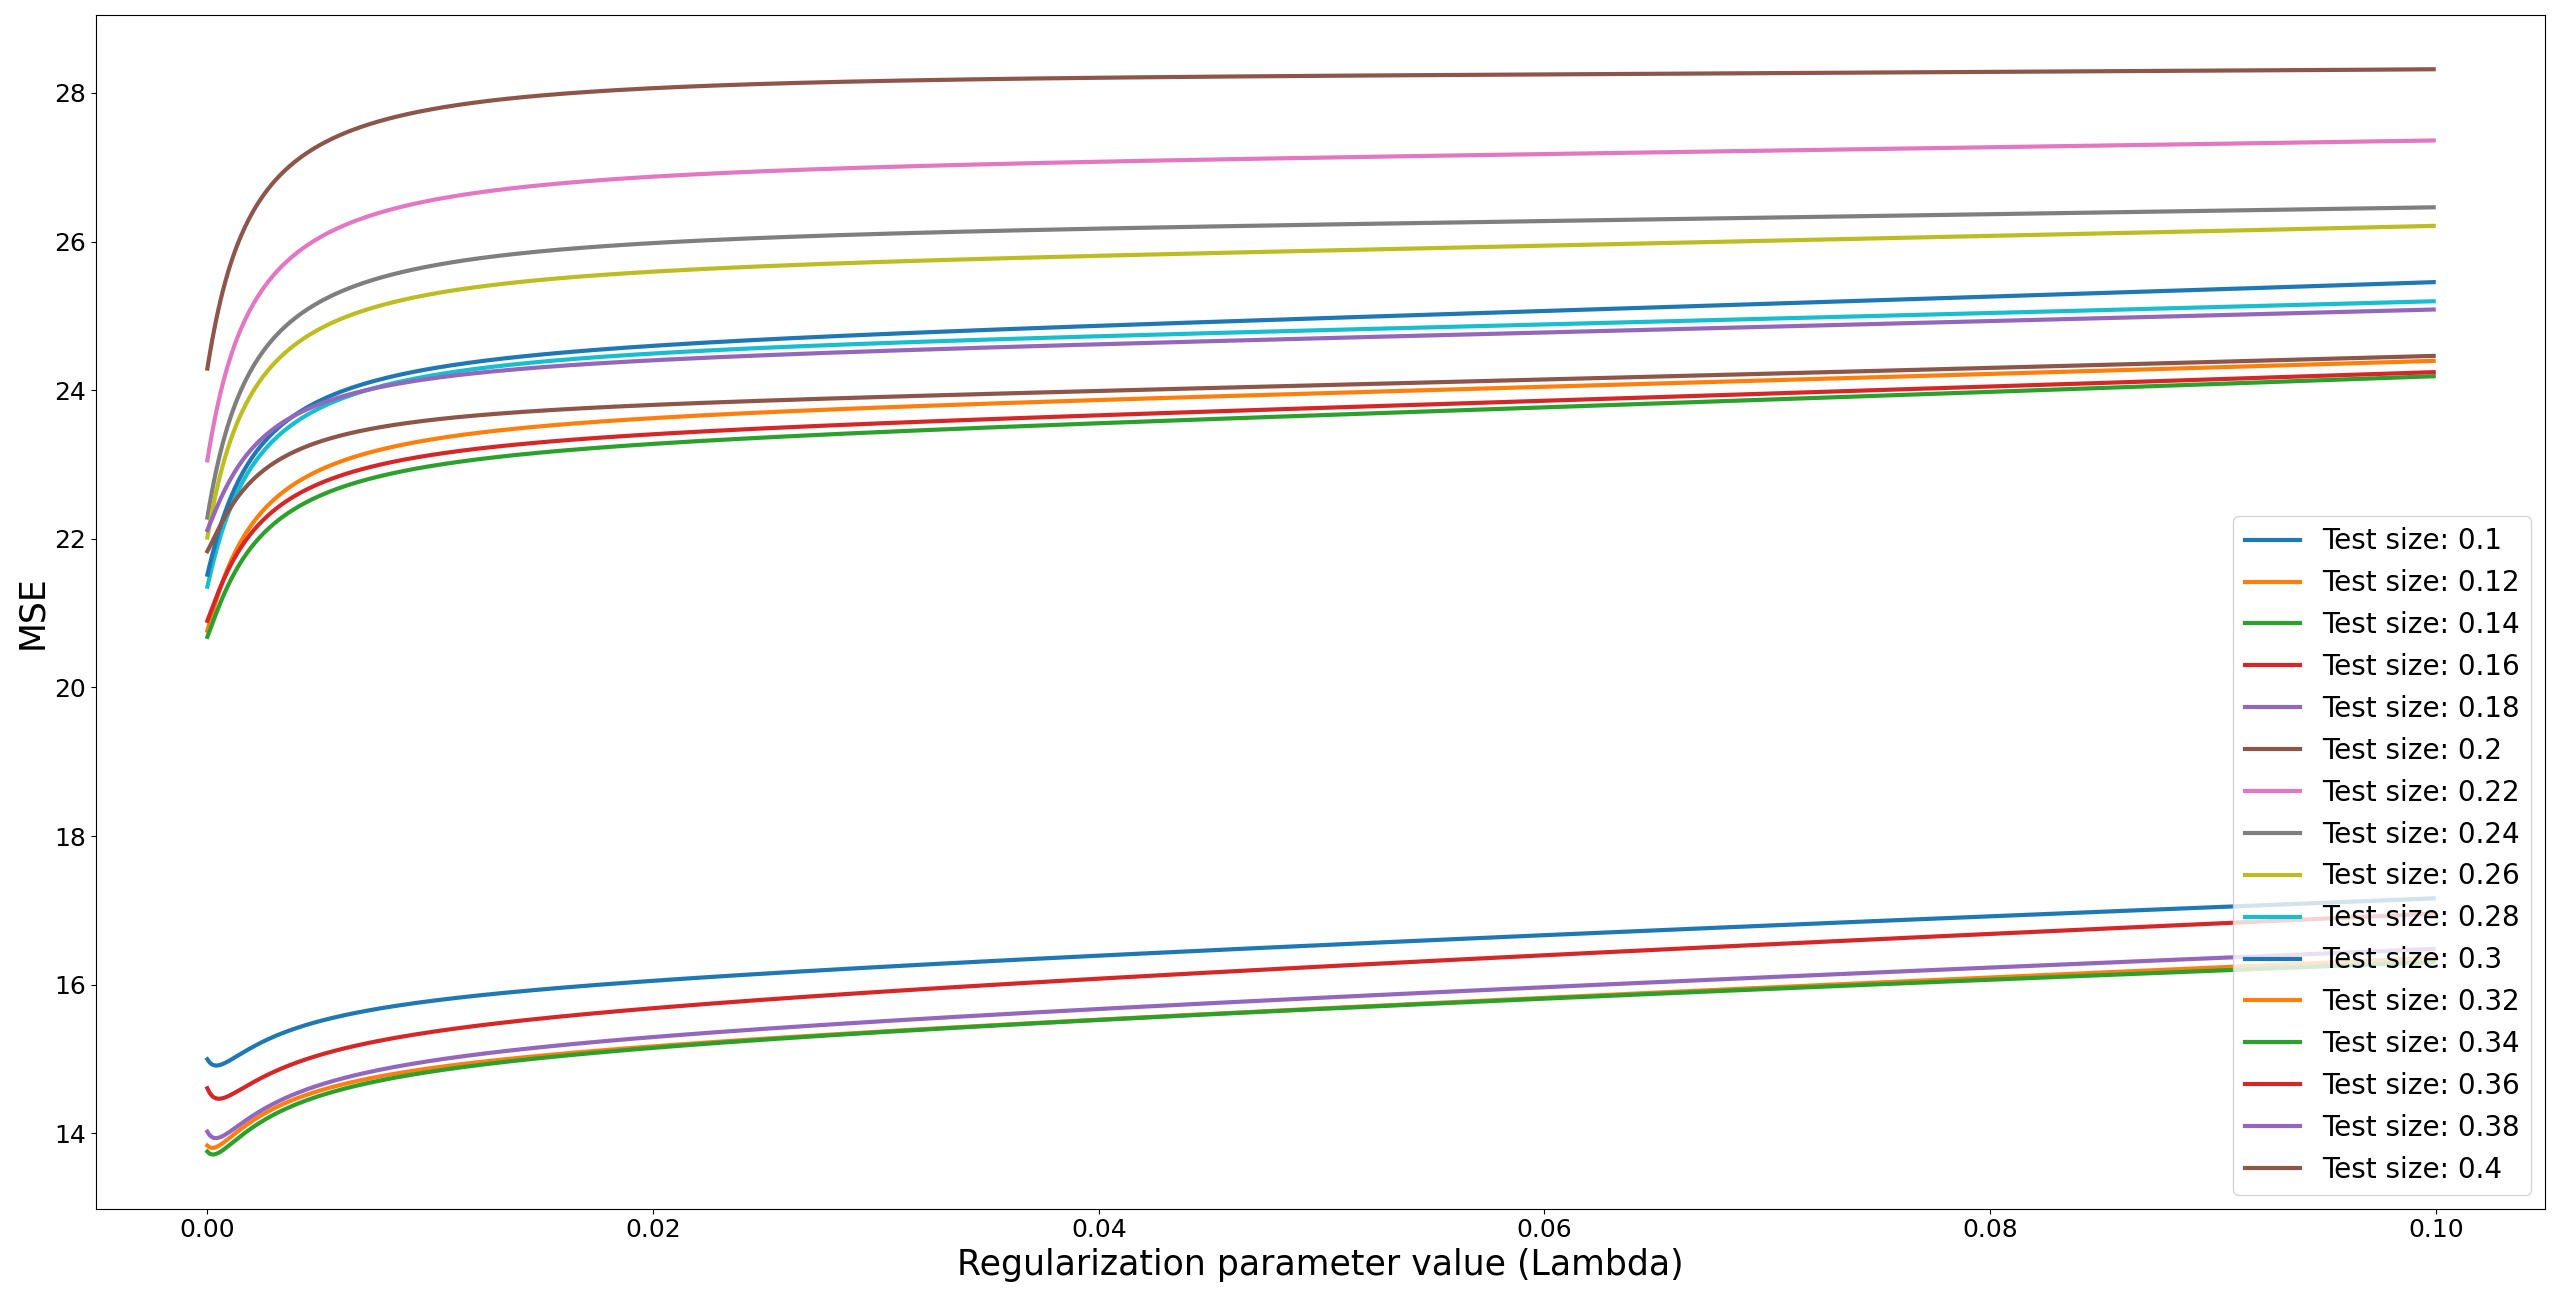
\includegraphics[width=\textwidth]{images/grid_search_w1.png}
\end{center}
\caption{Test Set MSE after Grid Search over train-test split range (0.1 to 0.4 w/ 0.02 step) \& regularization parameter range (0 to 0.1 w/ 0.0001 step)}
\end{figure}

\begin{figure}[H]
\begin{center}
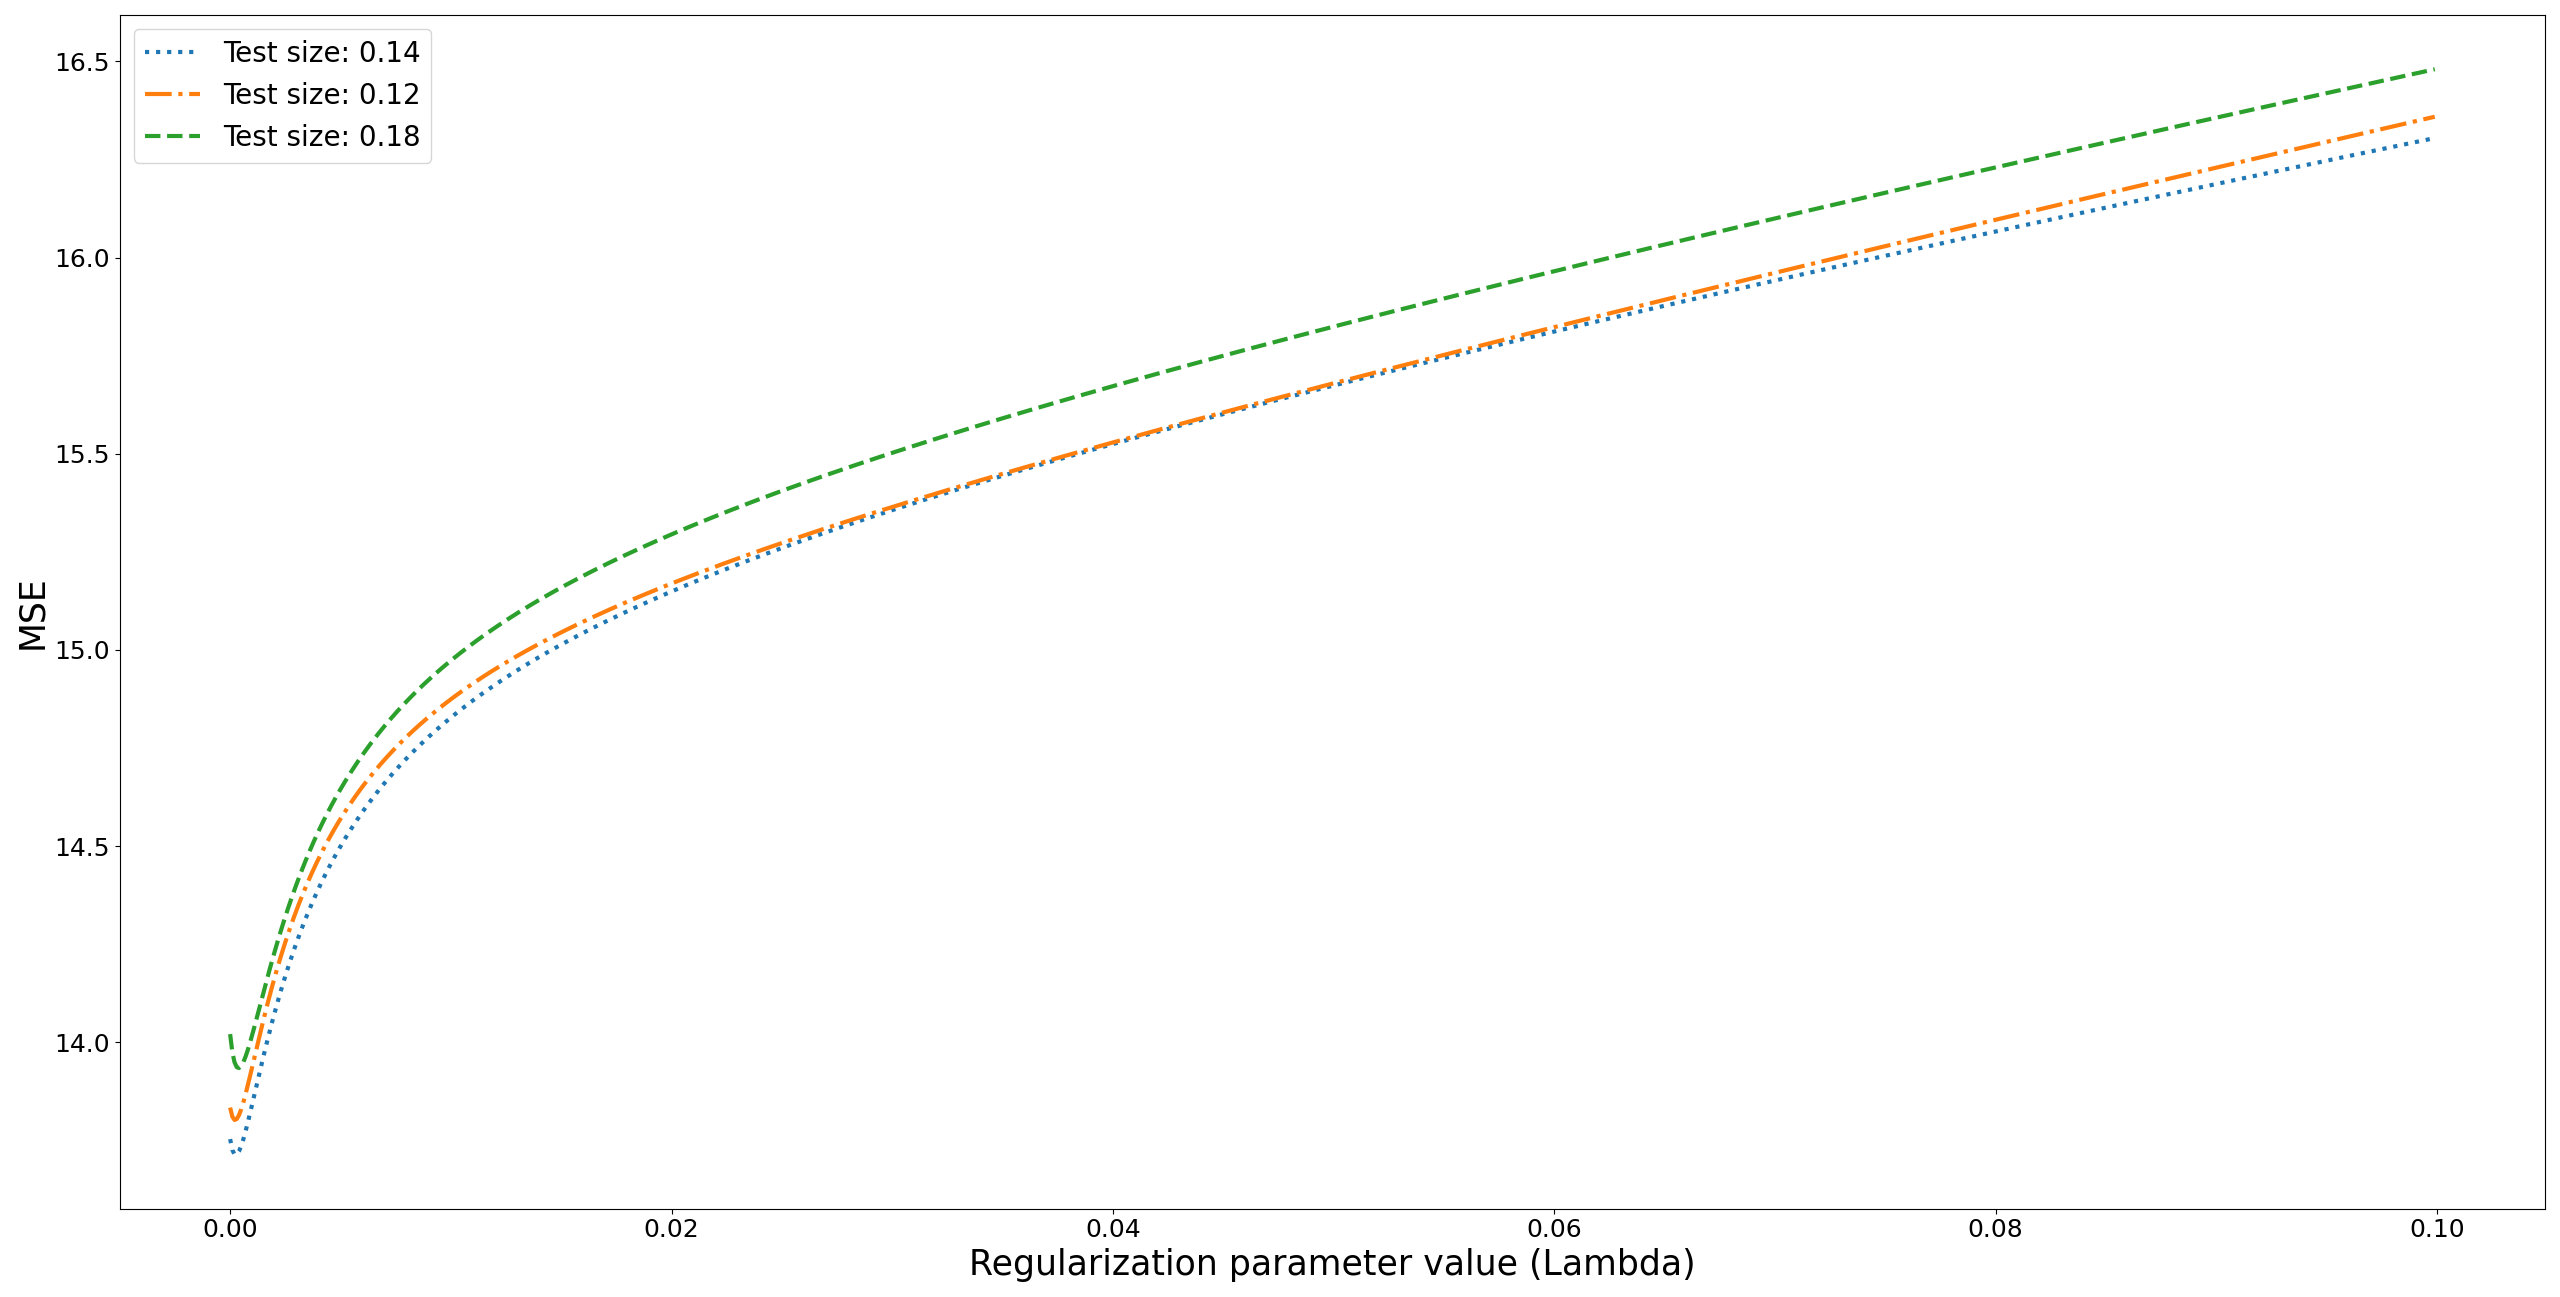
\includegraphics[width=\textwidth]{images/grid_search_w1_best3.png}
\end{center}
\caption{Best 3 Test Set MSE after Grid Search over train-test split range (0.1 to 0.4 w/ 0.02 step) \& regularization parameter range (0 to 0.1 w/ 0.0001 step)}
\end{figure}

\begin{figure}[H]
\begin{center}
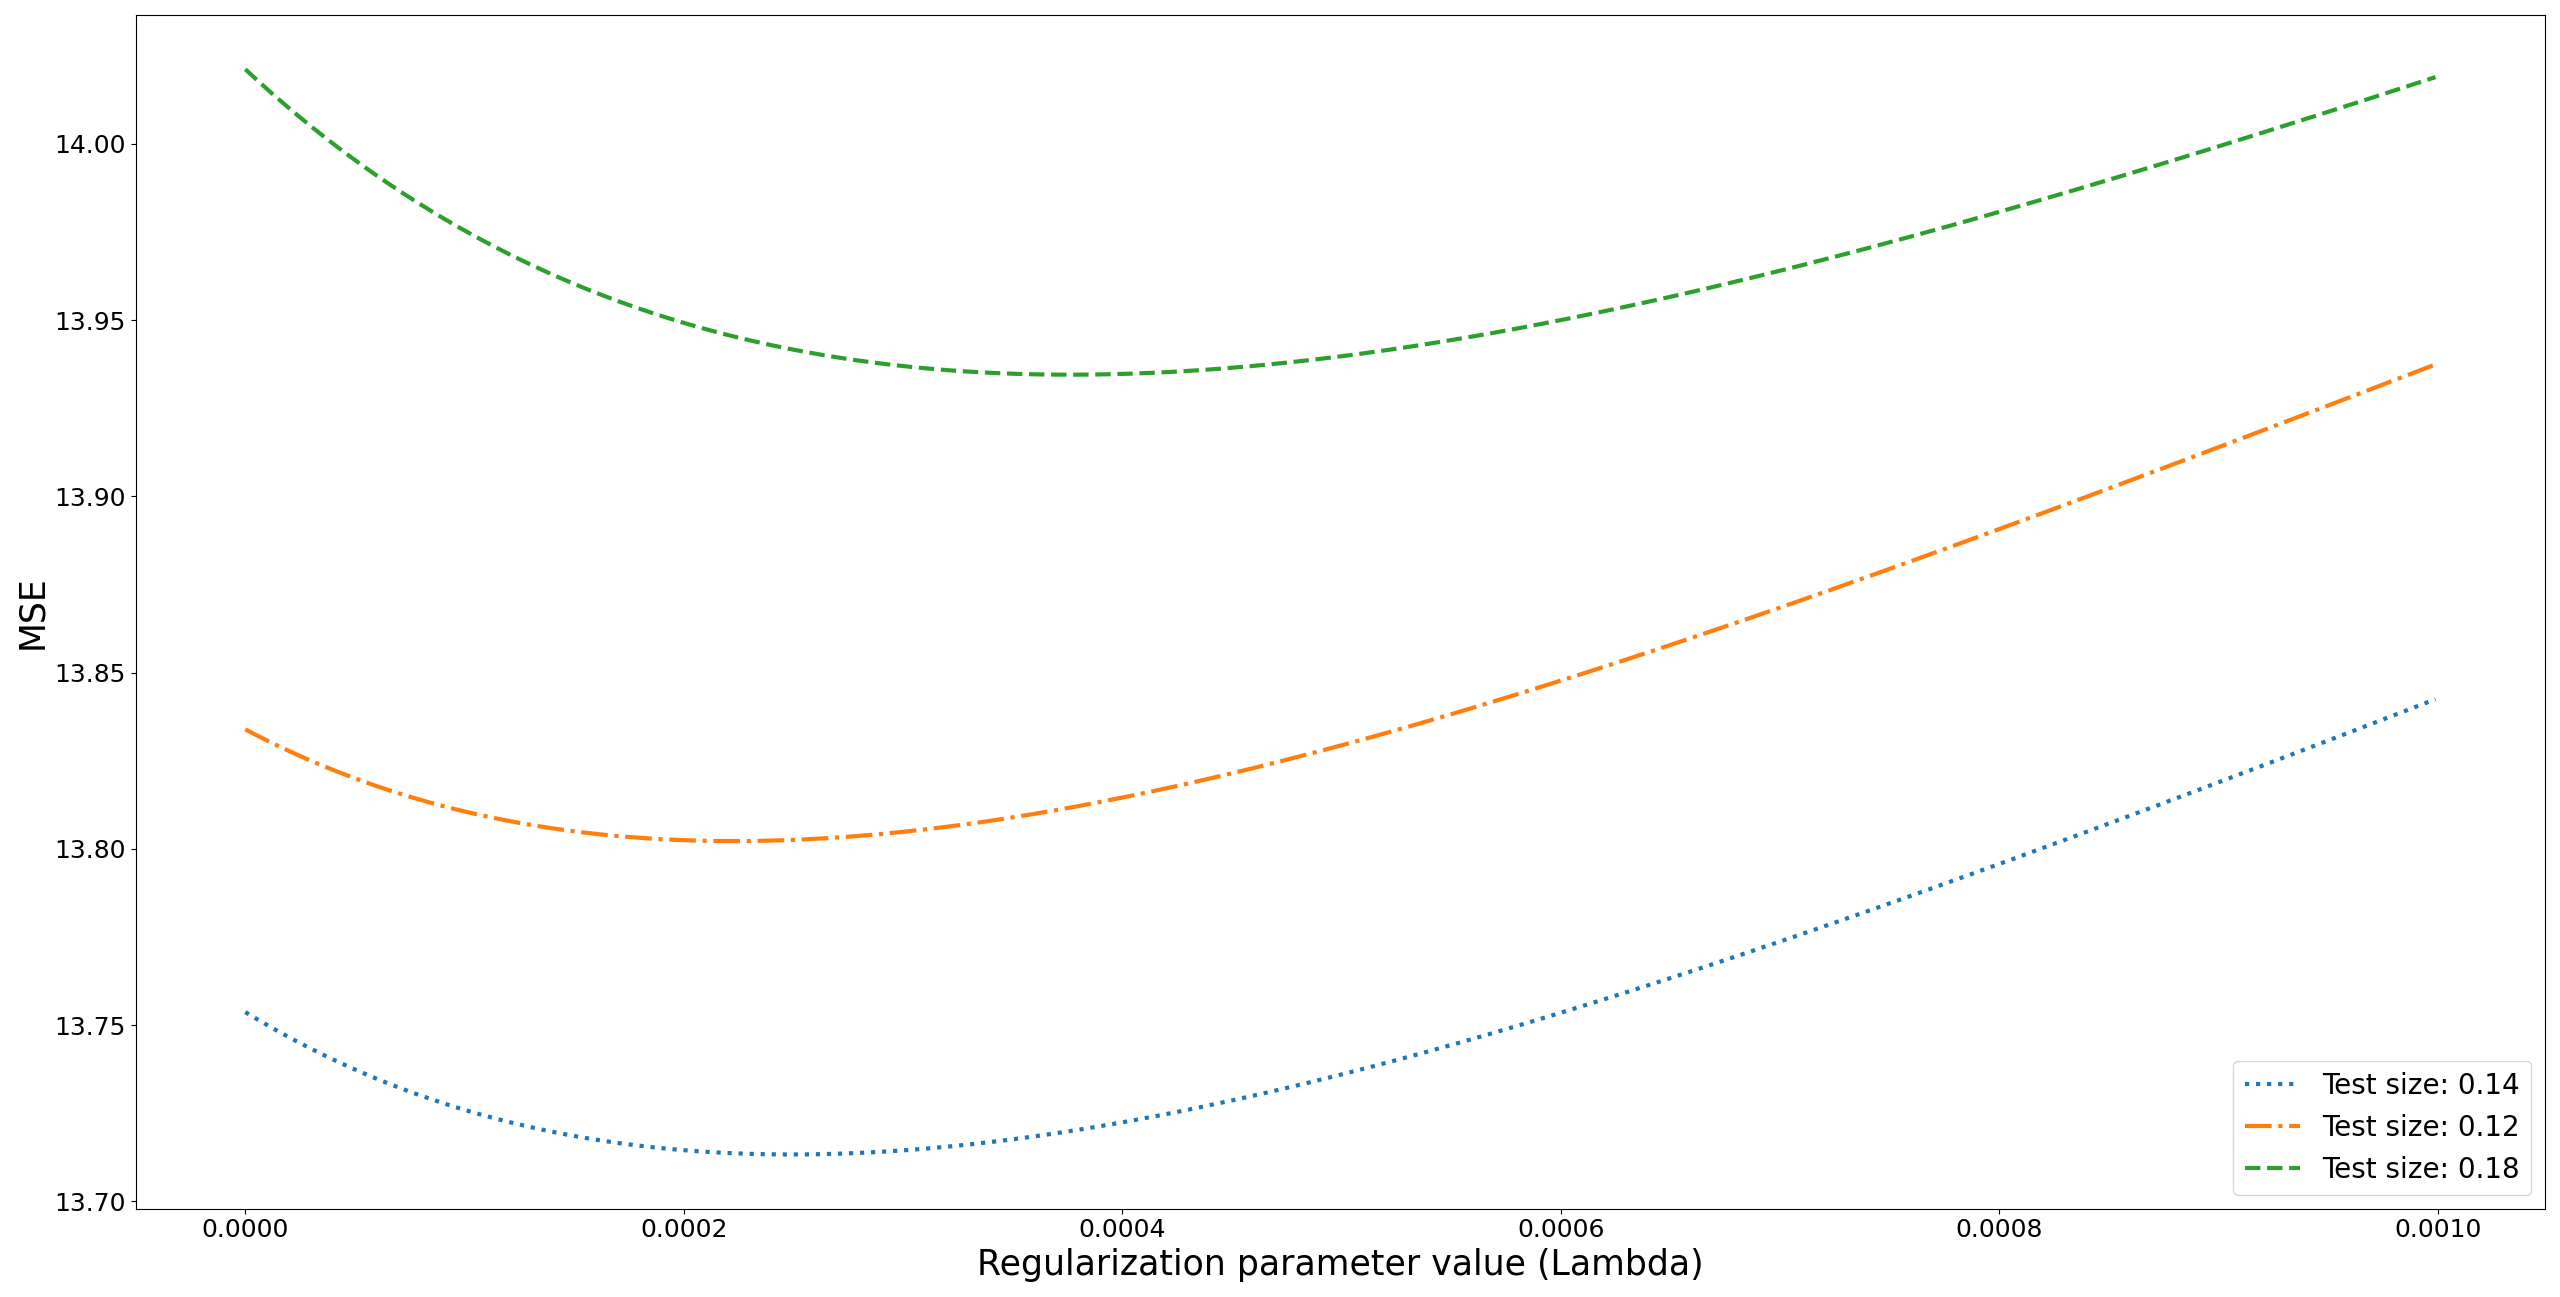
\includegraphics[width=\textwidth]{images/grid_search_w1_best3_focus.png}
\end{center}
\caption{Best 3 Test Set MSE from Figure 2 with a zoom on the regularization parameter range (0 to 0.001 w/ 0.000001 step)}
\end{figure}

\subsection*{II.6} 

We saw that there exist non-zero regularization parameters $\lambda$ such that Ridge Regression outperforms Ordinary Least Squares
with regards to predicting over the test set. I.e., Ridge Regression can have a better generalization capacity than OLS. Based
on these results, we can state the following hypothesis:

\textcolor{OliveGreen}{There exists a hyperparameter mix for Ridge Regression that is better than Ordinary Least Squares in terms 
of generalization error.}

\subsection*{II.7} 

The method we used above can be characterized as an exhaustive method: we try to exhaust all possibilities by
performing a Grid Search over all our hyperparameters of interest with as small a stepsize as possible. This
solution is not efficient, however, as it grows exponentially with the number of hyperparameters such that:
$${time}\,{complexity}=O(n^m)$$
Given:
\begin{itemize}
    \item $n$, the number of elements in the range of one hyperparameter (e.g. for Figure 1, we had 1,000
    elements in our regularization parameter range)
    \item $m$, the number of hyperparameters (e.g. for Figure 1, we had 2 hyperparameters)
\end{itemize}
\textbf{Note}: We abstracted out the additional time complexity of the underlying training process that we calculated in \textbf{I.11}.

If we search over a single hyperparameter (e.g. the regularization parameter $\lambda$) we reduce the relative time complexity to $O(n)$. 

Furthermore, we cannot say that this process is optimal, especially in the case of the Boston dataset. Indeed, as it is a small dataset,
performing a given train-test split over it might yield a biased mix of datapoints that would impede our goal: finding the model with the 
best generalization error. As such, we might be interested in another method: Cross-Validation.

\underline{1. Setting a new goal: minimizing an Information Criteria/the Tikhonov Factor}

The first step of this approach is to pick the regularization parameter $\lambda$ by minimizing an information criterion such as the 
Akaike Information Criterion (AIC), \cite{micha}.
$$AIC = log(\frac{SSR}{T})+\frac{2m}{T}$$
Given:
\begin{itemize}
    \item $SSR$, the sum of squared residual
    \item $T$, the number of elements in the dataset
    \item $m$, the number of parameters in the model
\end{itemize}

Another criterion we can select for minimization is the Tikhonov Factor, \cite{wikipedia_2021}:
$$G=\frac{SSR}{\tau^2}=\frac{||X\hat{W}-y||^2}{[{Transpose}[I-X(X^TX+\lambda^2I)^{-1}X^T]^2}$$
Given:
\begin{itemize}
    \item $SSR$, the sum of squared residual
    \item $\tau$, the effective number of degrees of freedom
\end{itemize}

Using a information criterion or factor, it has been shown that the optimal parameter can be found via a 
Leave-One-Out Cross Validation process, \cite{ridge}.

\underline{2. Performing a Leave-One-Out Cross-Validation:}

This approach tries to find $\lambda$ from a set of candidate values. The cross-validation process algorithm is the following:

\begin{algorithm}[H]
\SetAlgoLined
% \KwResult{Write here the result }
 Declare a parameter space for $\lambda$\;
 Declare a fixed number of folds $k$\;
 \For{<parameter $\lambda$> in [Parameter Range]}{
    \For{<k> in [1:k]}{
        Store $k$-th fold\;
        Compute $w$\;
        Compute predictions on $k$-th fold\;
        Compute Sum of Squared Residuals ($SSR$)\;
    }
    Compute the mean of $SSRs$ (${Mean}_{SSR}$) for a given parameter $\lambda$\;
 }
 Pick $\lambda$ that satisfies $\underset{\lambda}{argmin\,\,}{{Mean}_{SSR}}$\;
 \caption{K-Fold Cross-Validation Algorithm, \cite{micha}}
\end{algorithm}

\underline{3. Optimality}

Cross-validation is based on our first exhaustive method. However, the training process (computing $w$) must 
be repeated for each k-fold, implying a computational complexity of:
$${time}\,{complexity}=O(k*n^m)$$
Given:
\begin{itemize}
    \item $n$, the number of elements in one hyperparameter range (i.e. our regularization parameter 
    $\lambda$)
    \item $m$, the number of hyperparameters (e.g. for Figure 1, we had 2 hyperparameters)
    \item $k$, the number of folds used in the cross-validation process
\end{itemize}
As such, the process is more computationally expensive albeit only linearly so (by a factor of $k$ which, 
depending on its size might be relatively small). However, given the theoretical basis previously stated, 
this process might yield a more optimal regularization parameter $\lambda$. 

\textbf{Note}: We would have no guarantee that it will be the most optimal $\lambda$ value. Rather, we will have 
a high certainty that it will be more optimal than a $\lambda$ parameter obtained via our first, exhaustive method.

To summarize:

\textcolor{OliveGreen}{We propose to use K-fold Cross-Validation in order to find an optimal regularization parameter 
$\lambda$ since the implementation has theoretical support. However, we must note that this solution only appears optimal
relative to our previous method (exhaustive parameter search via Grid Search). We did not provide proof that this process is
the most optimal overall. A caveat to this solution is its linearly more expensive computational complexity.}

\subsection*{II.8 (Code available in Appendix F, Main() func call in Appendix H)} 

\textbf{Note}: We could center our $Y$ variable (our series of ground truths), however we decide not to so as to offer 
better comparison visualization in the question \textbf{II.9}.

Given:
\begin{itemize}
    \item a regularization parameter $\lambda$ set to $0.1$ as an example to compute $\hat{w}^1$
\end{itemize}
We obtain:
$$\hat{w}^2\in\mathbb{R}^{13},\quad\hat{w}^2 = \begin{bmatrix}
-1.09e^{-01} \\ 3.84e^{-02} \\ -3.91e^{-02} \\ 9.98e^{-01} \\ 5.01e^{-01} \\ 3.37e^{+00} \\
-8.75e^{-03} \\ -1.20e^{+00} \\ 2.27e^{-01} \\ -1.38e^{-02} \\ -7.89e^{-01} \\ 1.25e^{-02} \\
1.25e^{-02} 
\end{bmatrix}\quad b\in\mathbb{R},\quad b\approx22.80$$

We obtain for the first five predictions on the test set:
$$30.50\quad 35.84\quad 14.38\quad 26.3\quad 21.15$$

We reiterate the method used with $\hat{w}^1$ in \textbf{II.5} and prior. As such, we find results similar to the one
displayed in Figures 1 and 2 (See Figures 4 and 5). Furthermore, by using $\hat{w}^2$ and $b$ we find the following 
three best results with the resulting minimizing regularization parameters $\lambda$:

\begin{center}
\begin{tabular}{ | c | c | c | c | } 
\hline
\textbf{Train-test split} & \textbf{Best MSE achieved with regularization parameter $\lambda$:} \\
\hline
0.88/0.12 & 0.001578 \\
\hline
0.86/0.14 & 0.001861 \\
\hline
0.82/0.16 & 0.004979 \\
\hline
\end{tabular}
\end{center}

\begin{figure}[H]
\begin{center}
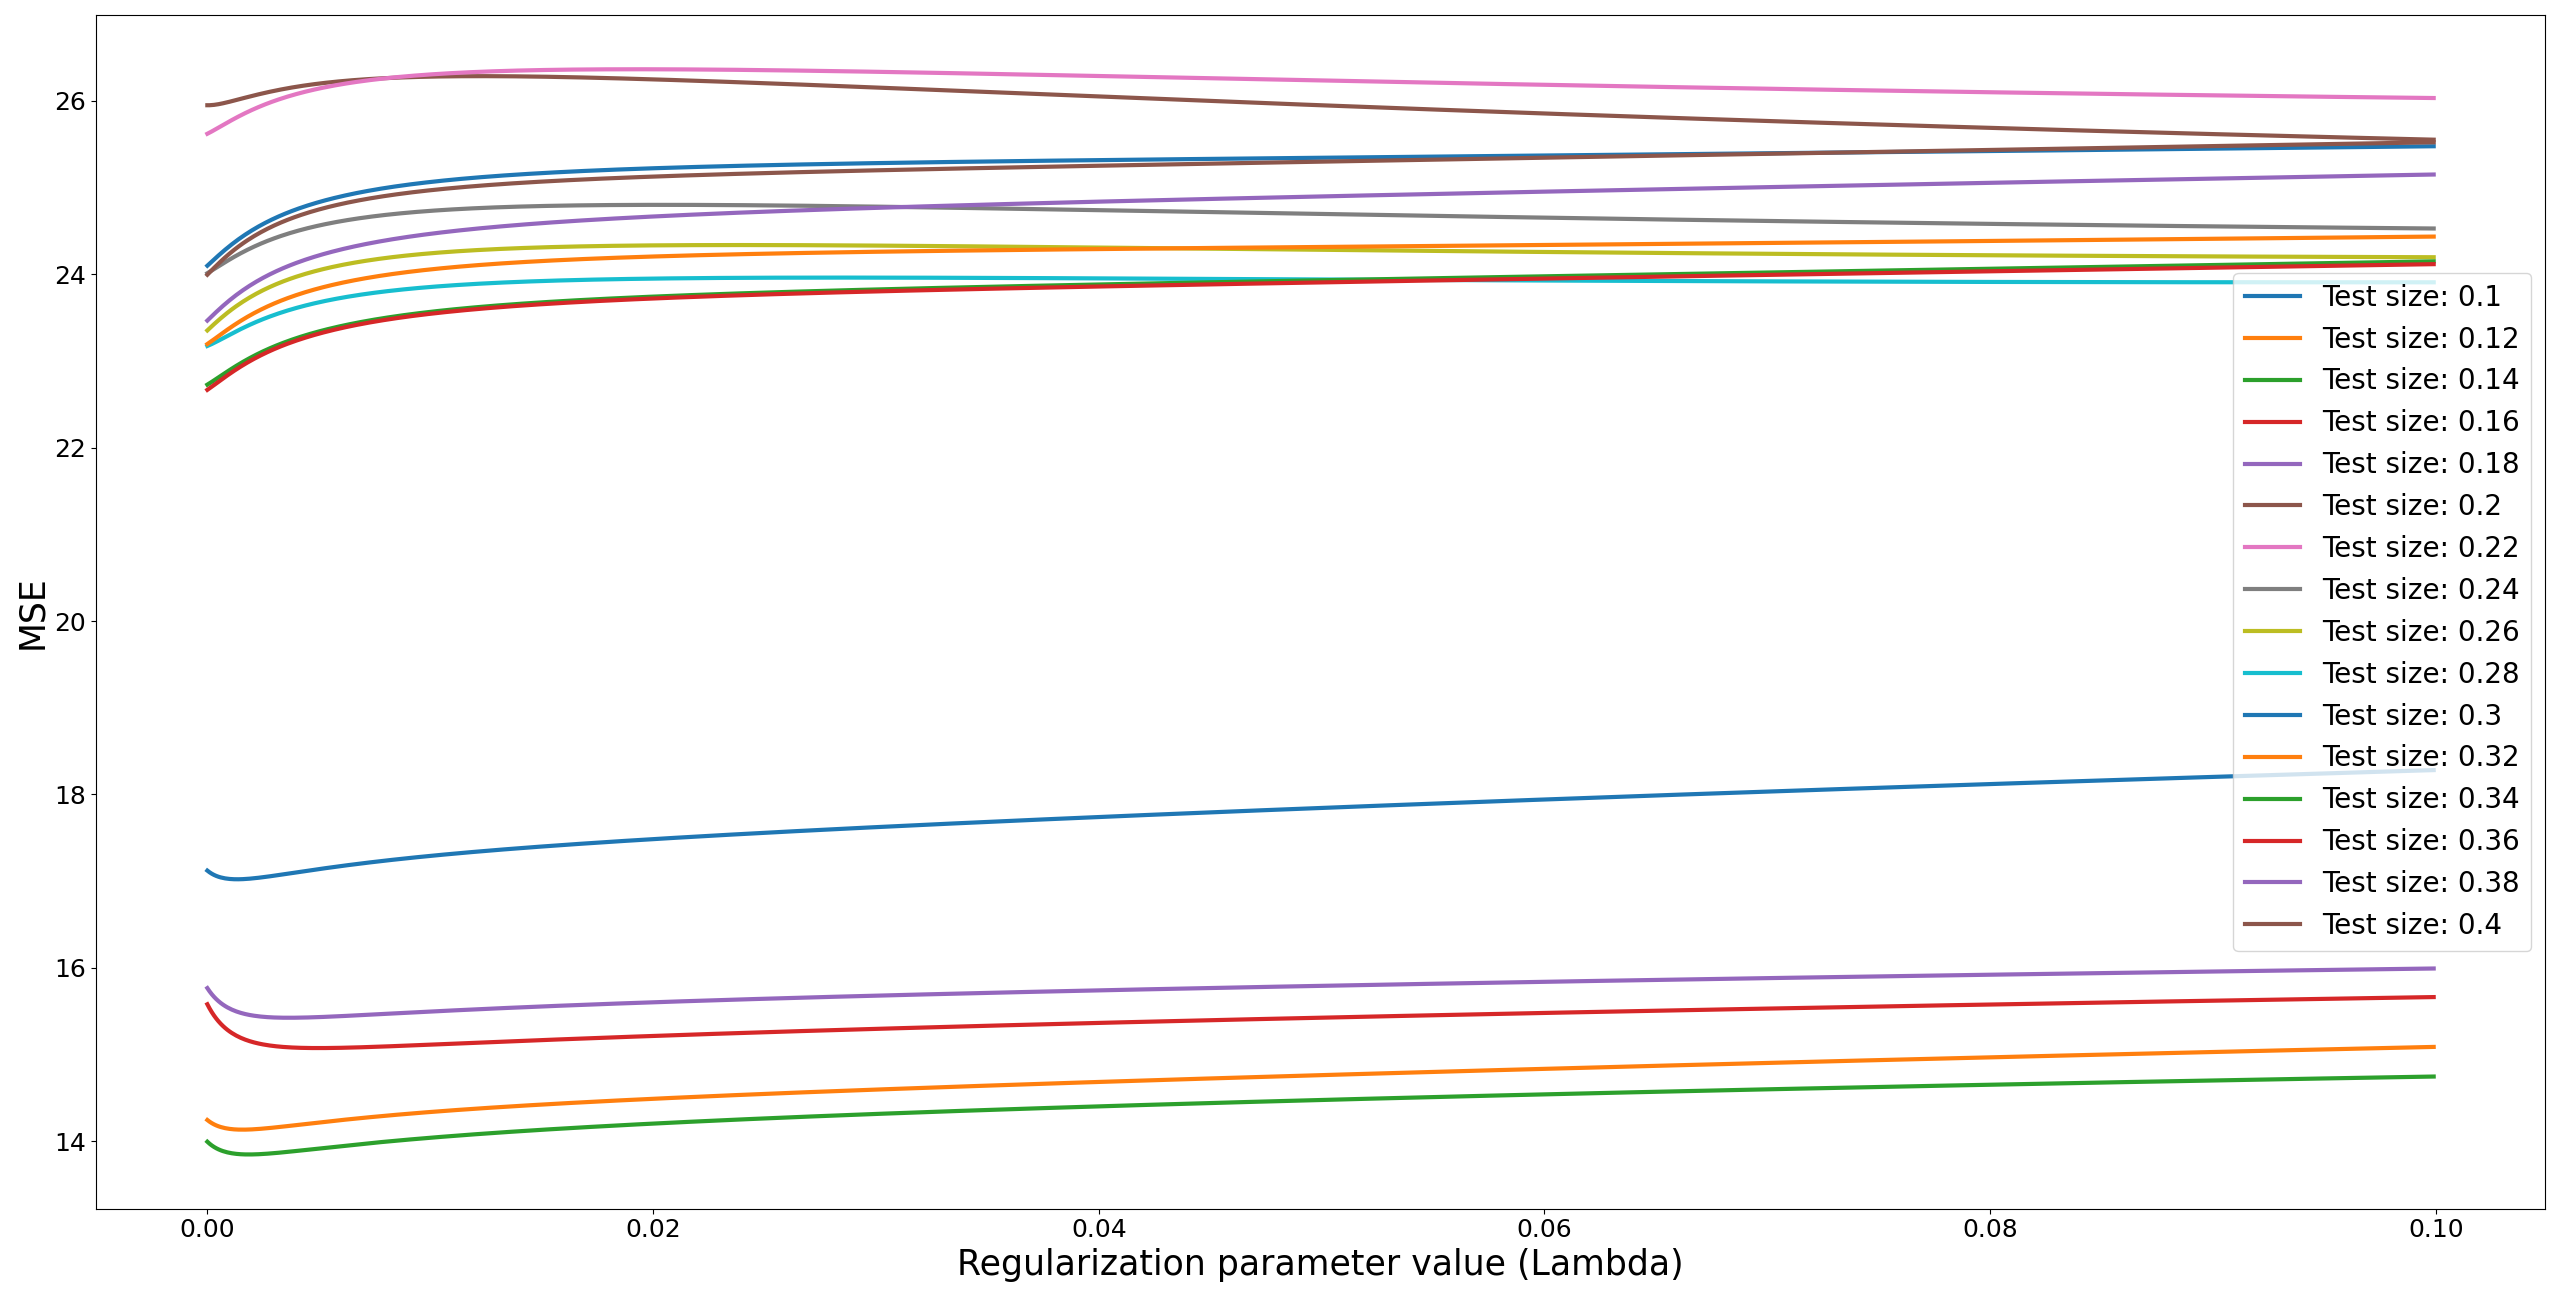
\includegraphics[width=\textwidth]{images/grid_search_w2.png}
\end{center}
\caption{Test Set (centered) MSE after Grid Search over train-test split range (0.1 to 0.4 w/ 0.02 step) \& regularization parameter range (0 to 0.1 w/ 0.0001 step)}
\end{figure}

\begin{figure}[H]
\begin{center}
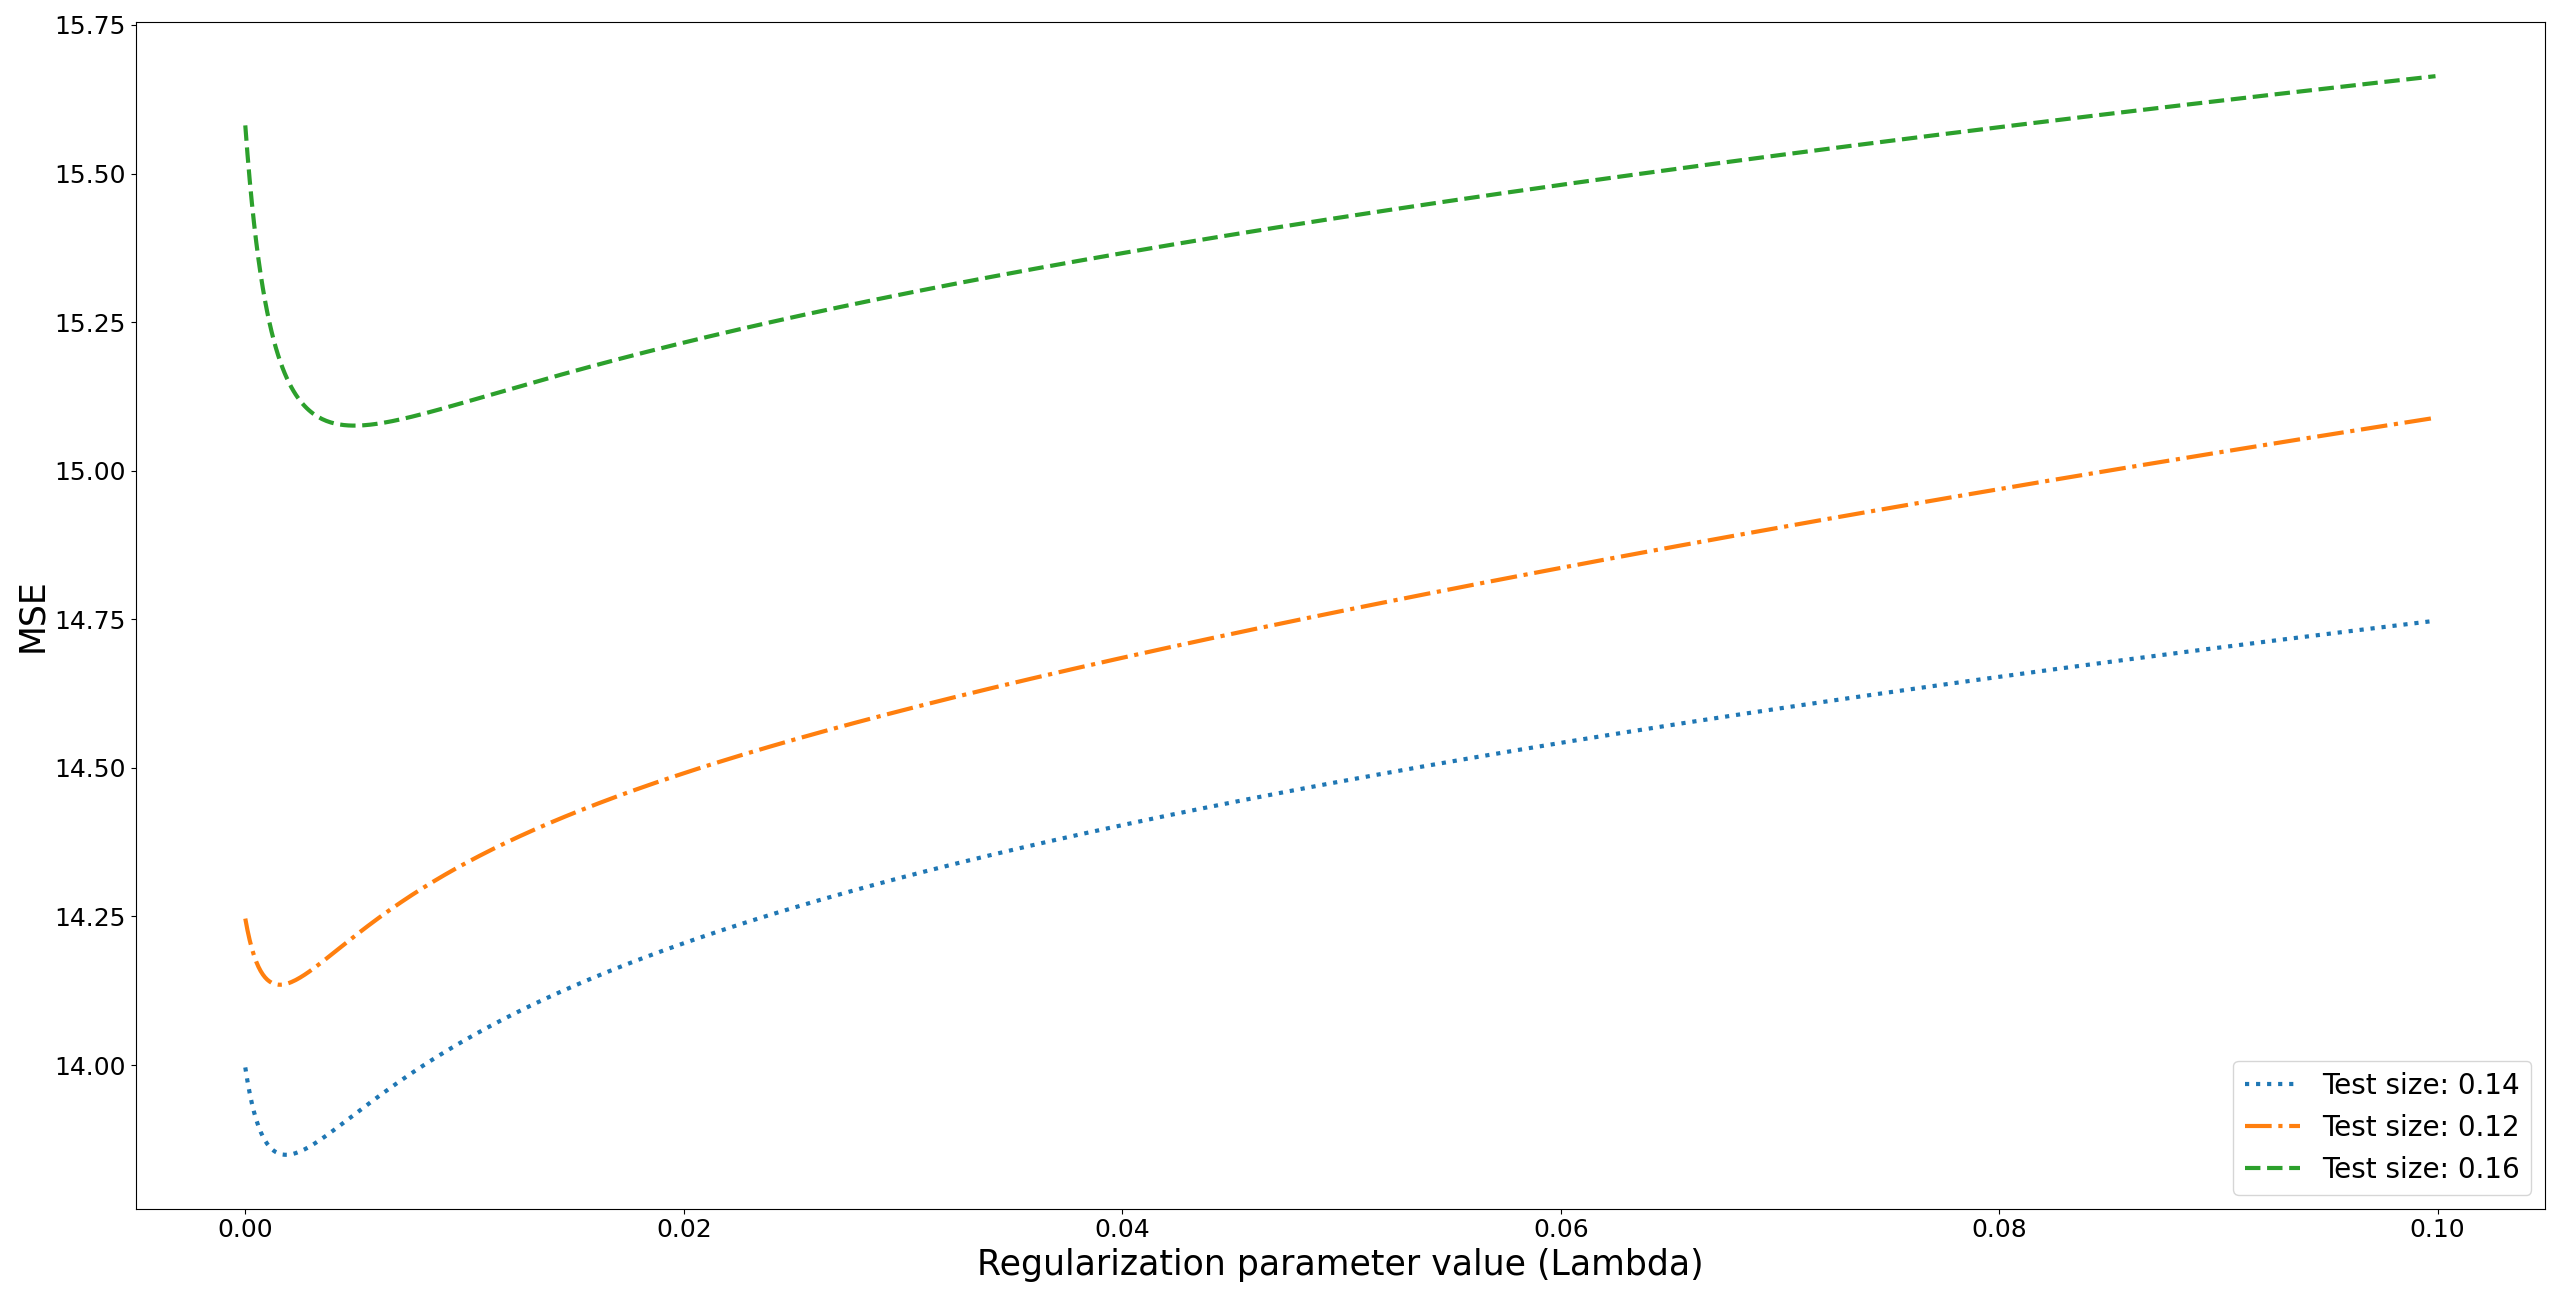
\includegraphics[width=\textwidth]{images/grid_search_w2_best3.png}
\end{center}
\caption{Best 3 Test Set (centered) MSE after Grid Search over train-test split range (0.1 to 0.4 w/ 0.02 step) \& regularization parameter range (0 to 0.1 w/ 0.0001 step)}
\end{figure}

\begin{figure}[H]
\begin{center}
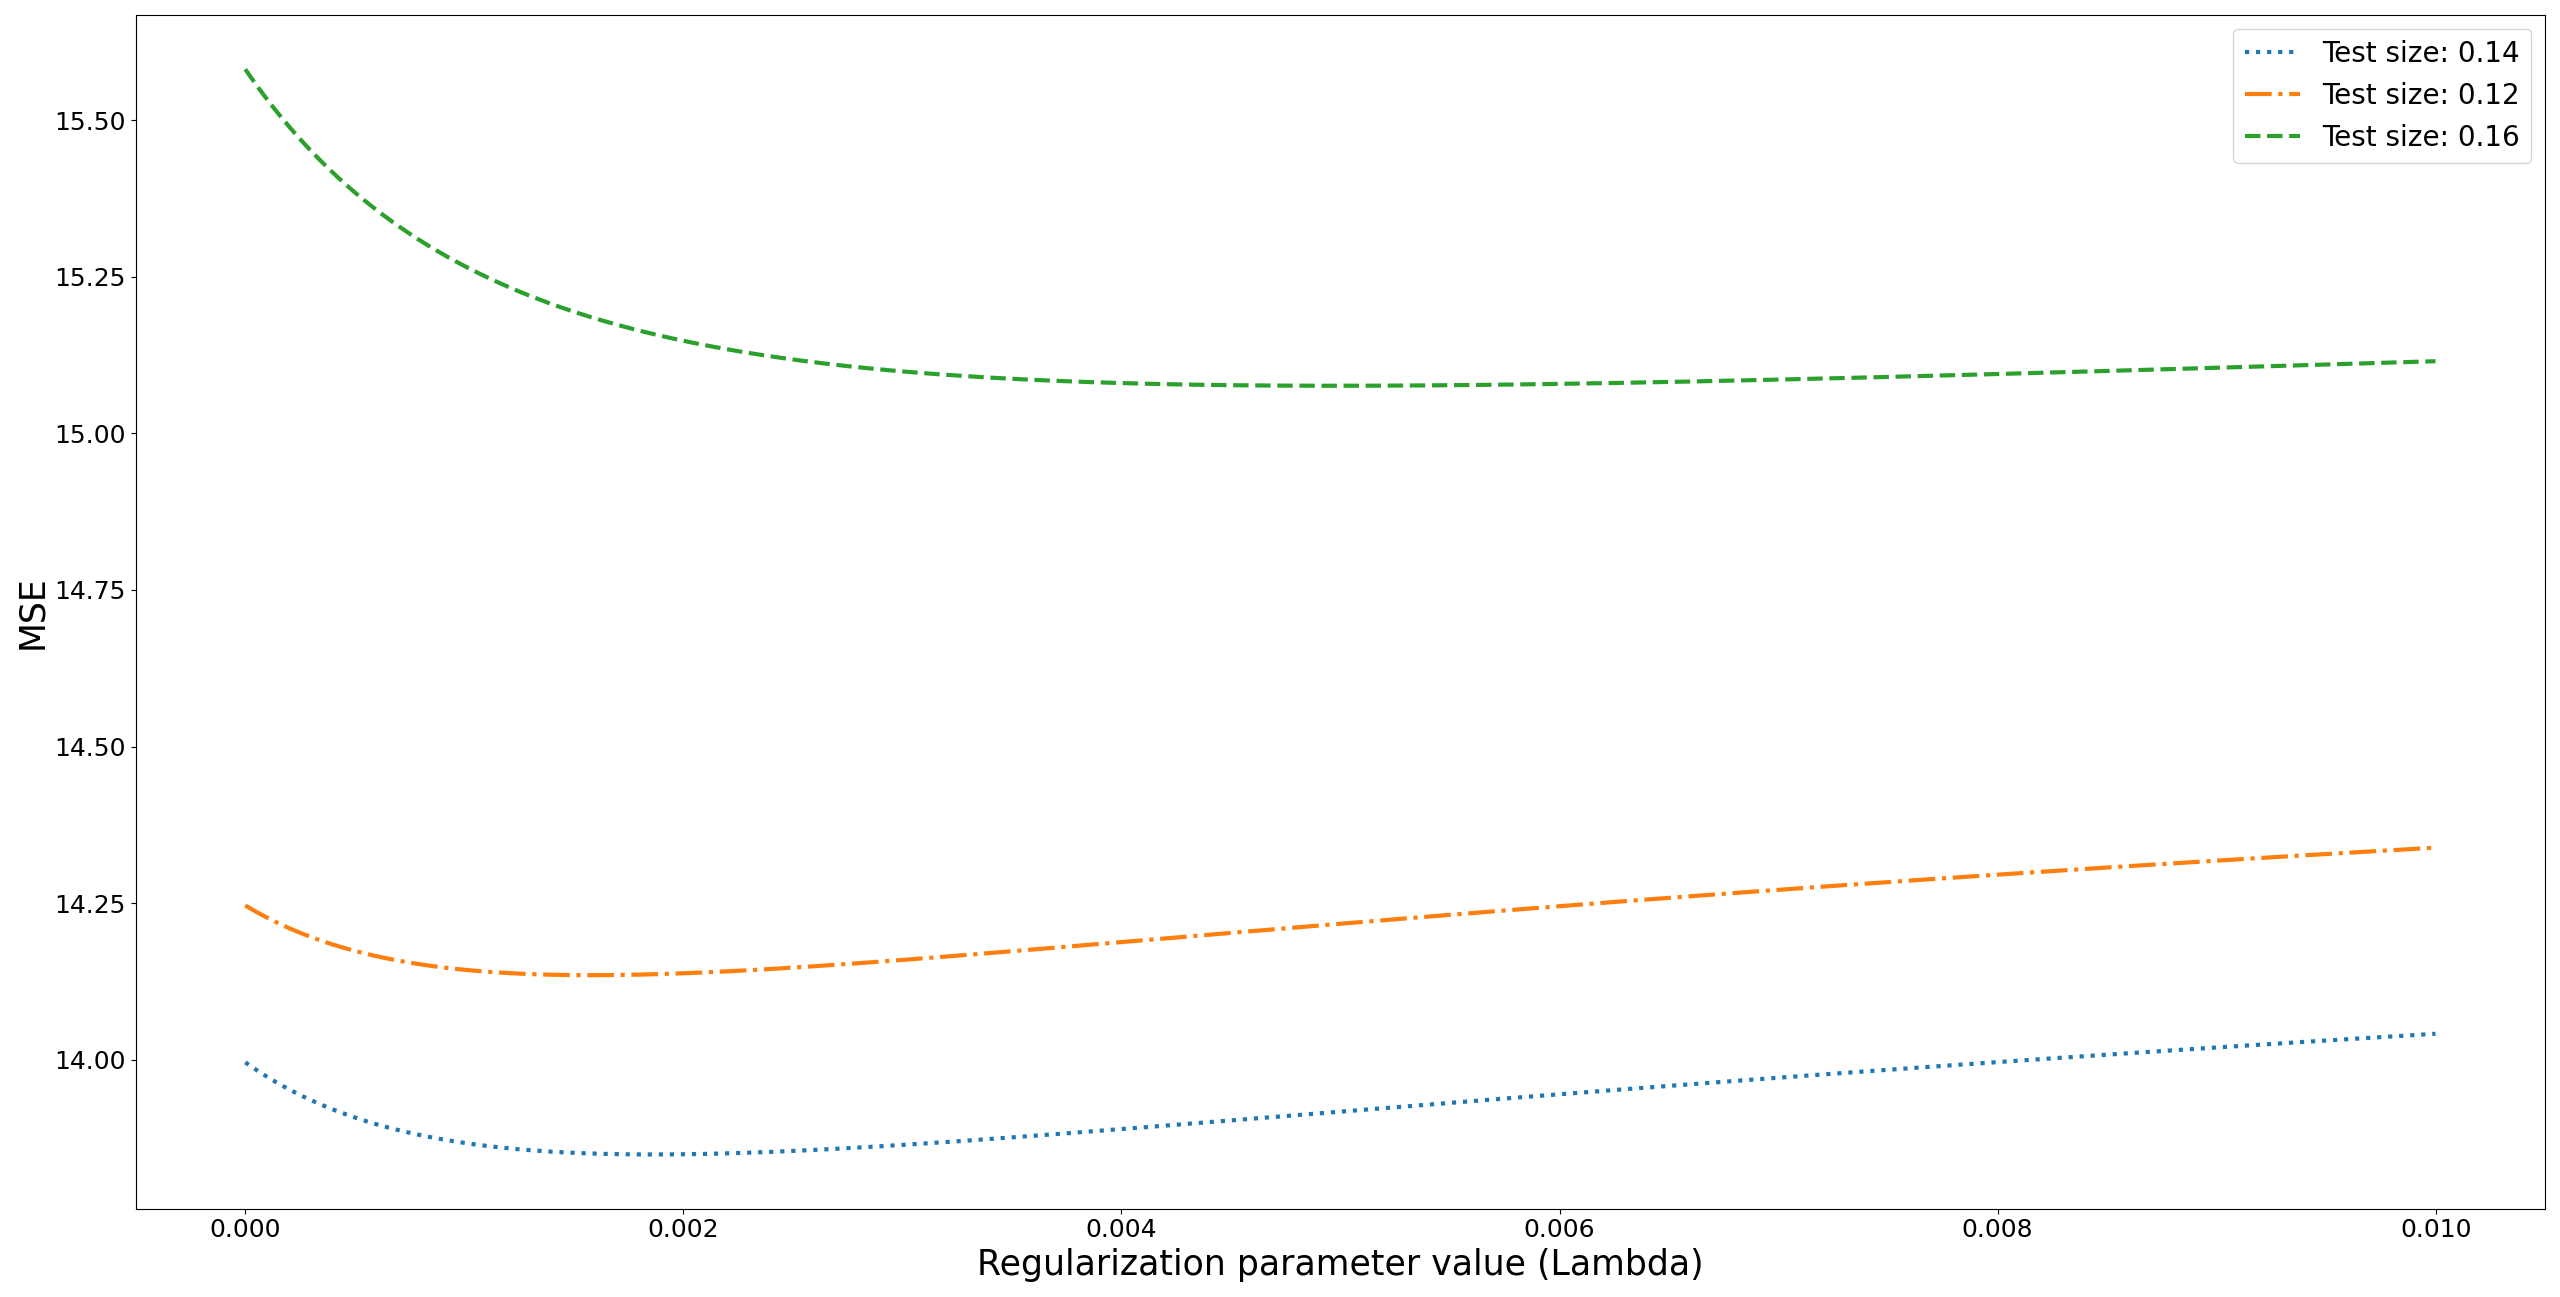
\includegraphics[width=\textwidth]{images/grid_search_w2_best3_focus.png}
\end{center}
\caption{Best 3 Test Set (centered) MSE from Figure 5 with a zoom on the regularization parameter range (0 to 0.01 w/ 0.000001 step)}
\end{figure}

\subsection*{II.9 (Code available in Appendix G, Main() func call in Appendix H)} 

Given:
\begin{itemize}
    \item a regularization parameter $\lambda$ set to $0.1$ as an example to compute $\hat{w}^2$
\end{itemize}
We obtain similar results between the two methods (computing $\hat{w}^1$, and $\hat{w}^2$ and $b$). Those similarities are made apparent 
in Figure 7 as the values predicted with each method are very clost to each other.

\begin{figure}[H]
\begin{center}
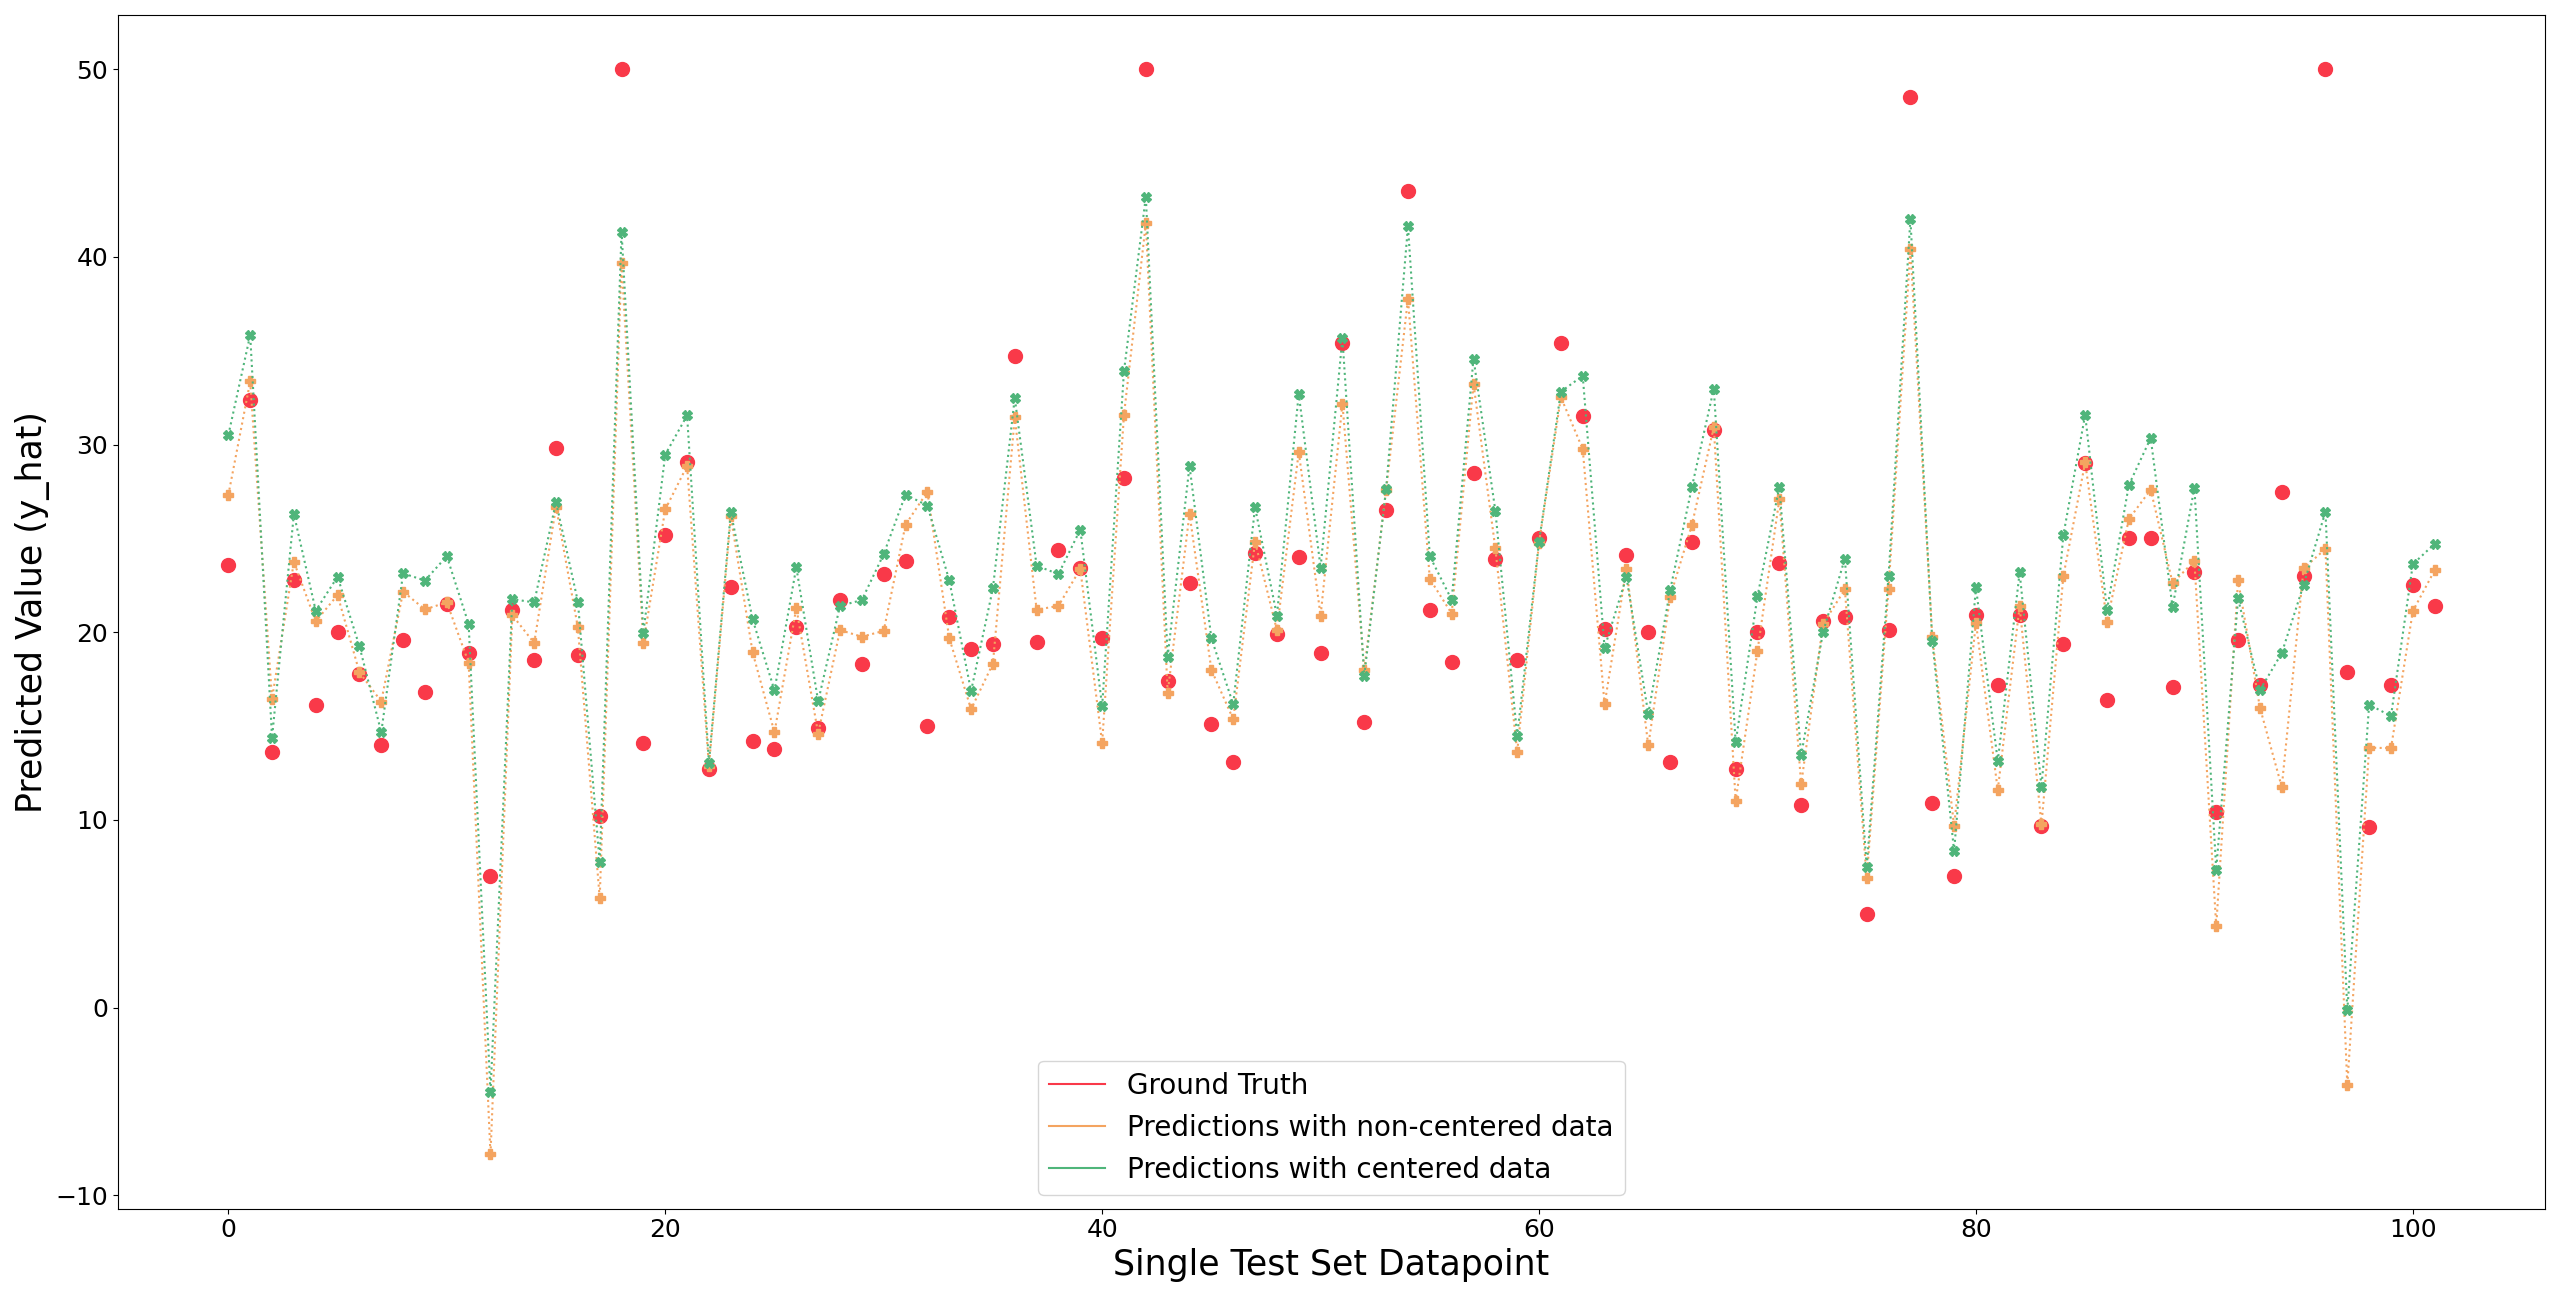
\includegraphics[width=\textwidth]{images/w1_w2_compare.png}
\end{center}
\caption{Comparison of the predictions computed with $\hat{w}^1$ and $\hat{w}^2$/$b$ with the ground truth $Y$ for the 
Test Set, given a 0.8/0.2 train-test split and regularization parameter $\lambda=0.1$}
\end{figure}

To summarize, we find that:

\begin{itemize}
    \item Both methods can lead to Ridge Regression models that outperform Ordinary Least Squares, given specific hyperparameter mixes 
    (in our case: train-test split/regularization parameter $\lambda$).
    \item Both methods find the train-test splits 0.88/0.12 and 0.86/0.14 among the three best splits (i.e. which yielded on average, 
    over the range of regularization parameters $\lambda$ used for Grid Search, the lowest mean of MSE scores).
    \item Both methods find the best regularization parameters in the range $]0; 0.005[$. Of note, the method with centered data 
    (i.e., computing $\hat{w}^2$ and $b$) finds relatively larger regularization parameters $\lambda$, by about one order of magnitude.
\end{itemize}

Next, we want to compare the predictions on the test set made by the two methods. To do so, we select one of the shared train-test splits
between the two methods (e.g. 0.86/0.14) and use their respective minimizing regularization parameter values (e.g. $\lambda_{\hat{w}^1}=0.000249$,
$\lambda_{\hat{w}^2}=0.001861$). As seen in Figure 8, the end predictions are consistently very close to one another between the two methods, 
if not overlapping.

\begin{figure}[H]
\begin{center}
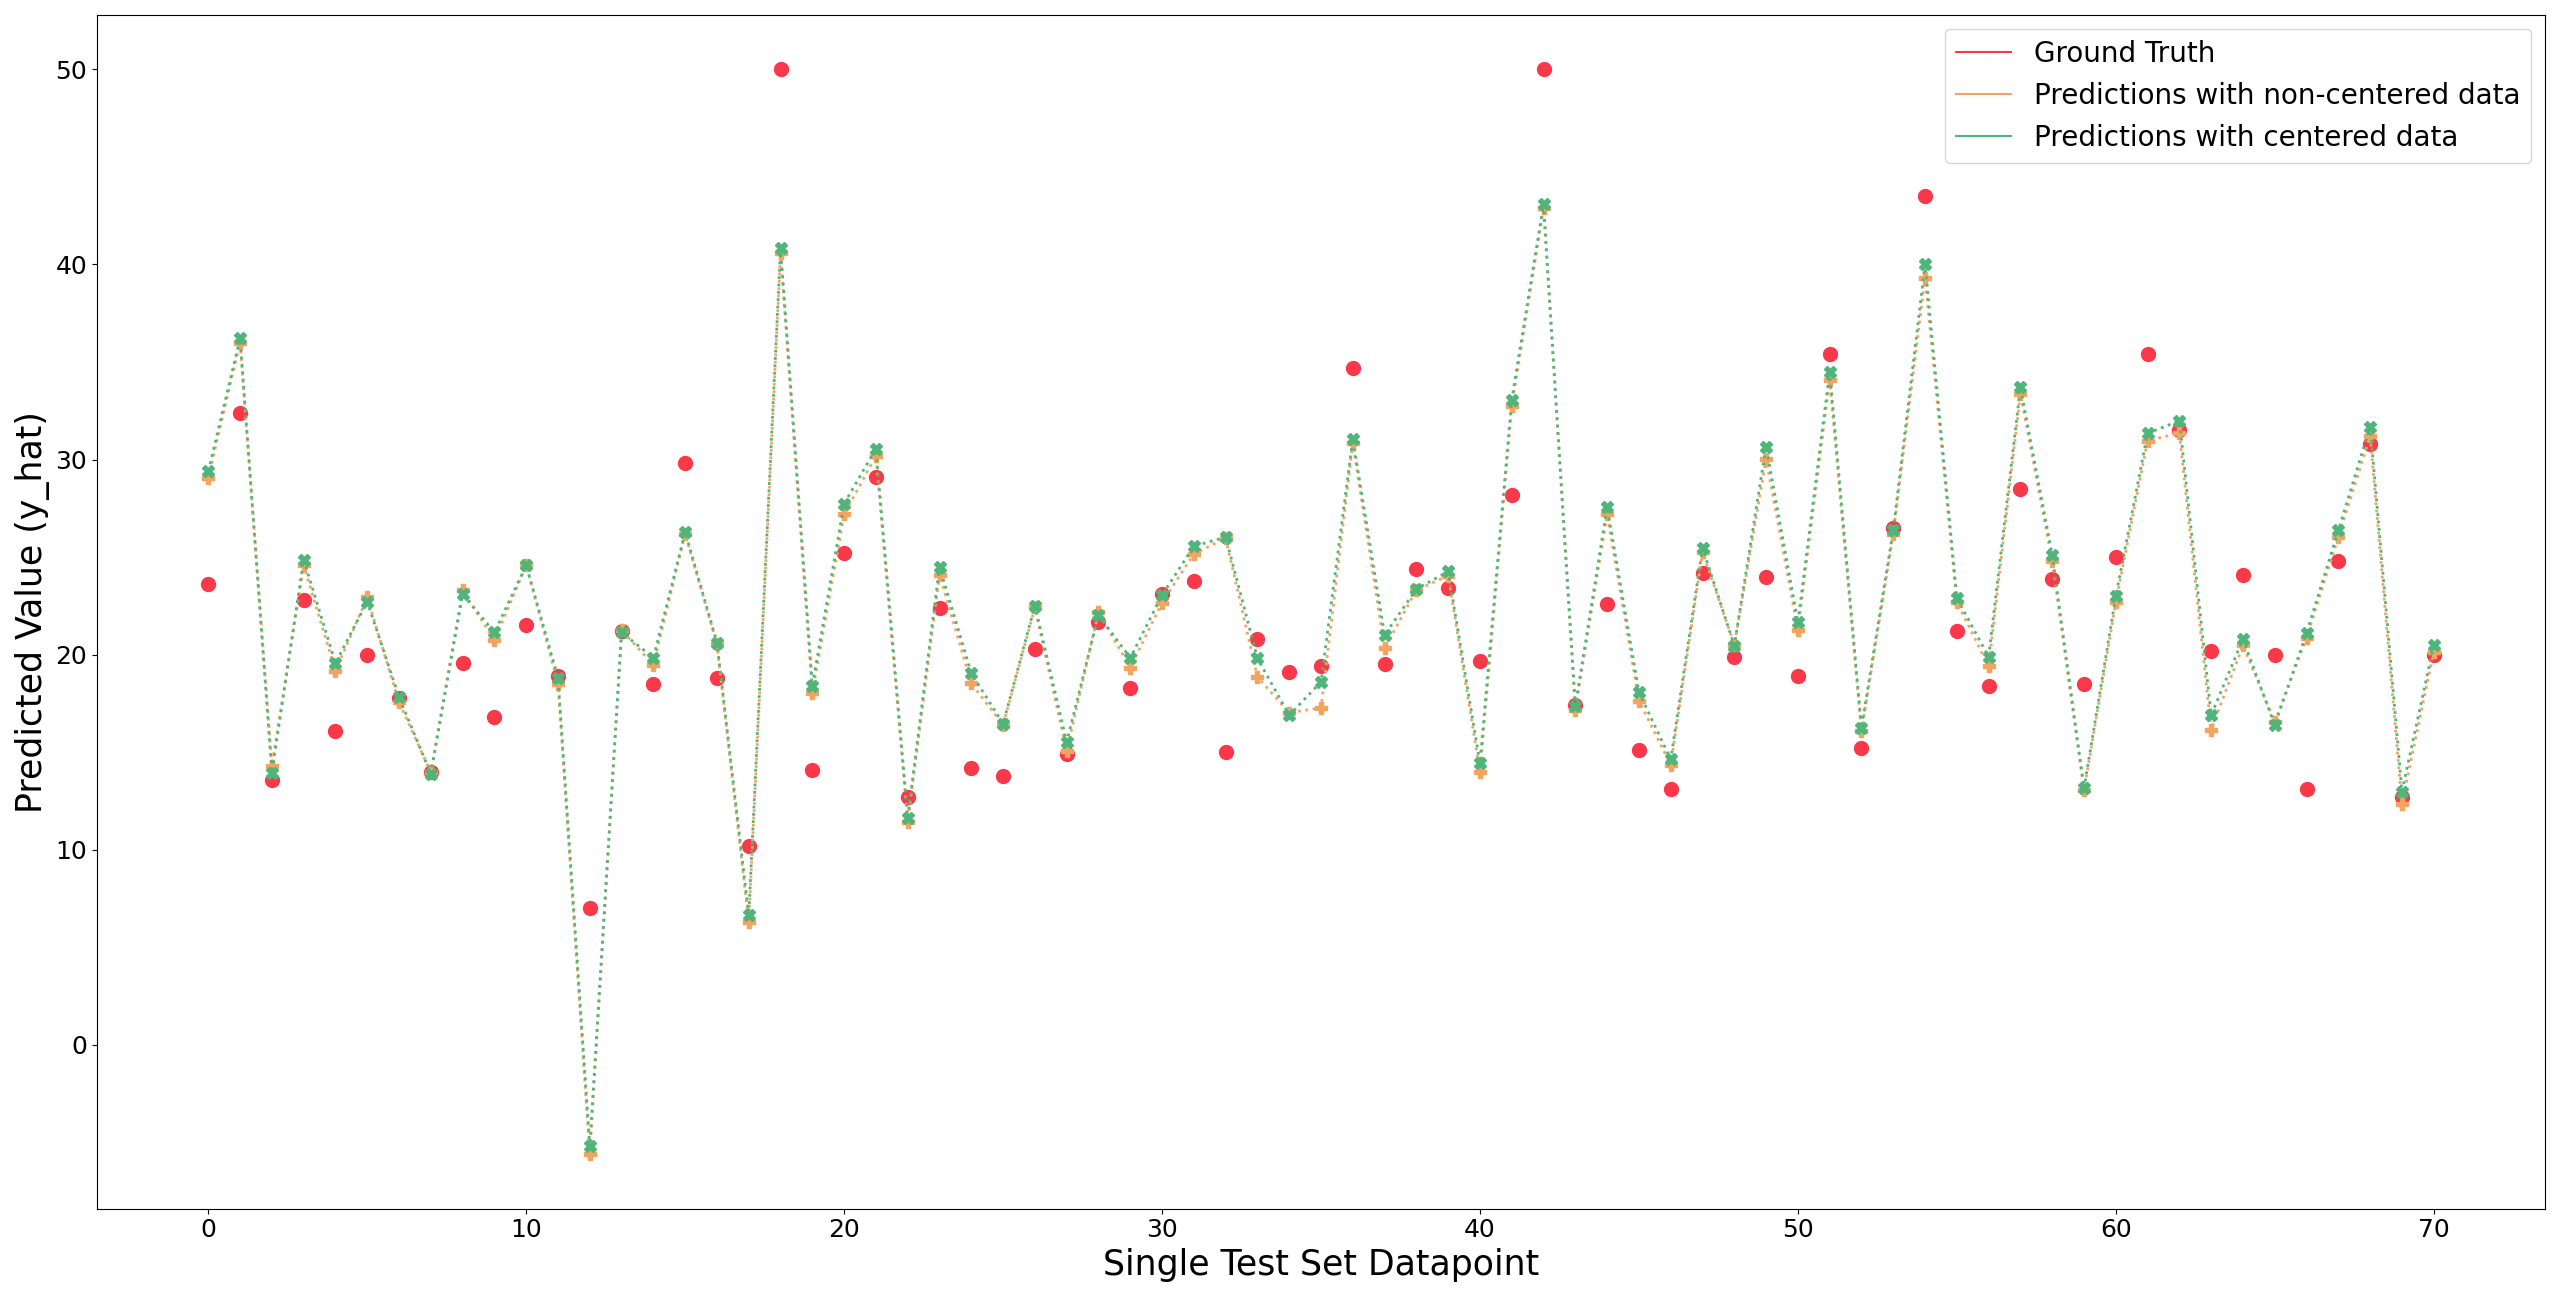
\includegraphics[width=\textwidth]{images/w1_w2_compare_best_regs.png}
\end{center}
\caption{Comparison of the predictions computed with $\hat{w}^1$ and $\hat{w}^2$/$b$ with the ground truth $Y$ for the 
Test Set, given a 0.86/0.14 train-test split and the regularization parameters $\lambda_{\hat{w}^1}=0.000249$ and 
$\lambda_{\hat{w}^2}=0.001861$}
\end{figure}
We conclude that:

\textcolor{OliveGreen}{The two methods seem to yield approximately similar predictions over the Boston Dataset as we showed in \textbf{Part 1} of this assignment.}

\subsection*{II.10} 

We refer to the \href{https://scikit-learn.org/stable/modules/generated/sklearn.linear_model.Ridge.html#sklearn.linear_model.Ridge}{\texttt{Sklearn} documentation}, 
\cite{sklearn_api}, for the \texttt{Ridge} model implementation.

The \texttt{Ridge} model implementation is found within the library \texttt{Sklearn.linear\_model}. Among \texttt{Ridge}'s initialization 
parameters we find the counterpart to our regularization parameter $\lambda$ in the class attribute/parameter \texttt{alpha}:
\begin{displayquote}
\texttt{alpha -- float, ndarray of shape (n\_targets,) --, default=1.0 \newline Regularization strength; must be a positive float. Regularization 
improves the conditioning of the problem and reduces the variance of the estimates. Larger values specify stronger regularization. Alpha corresponds 
to 1 / (2C) in other linear models such as LogisticRegression or LinearSVC. If an array is passed, penalties are assumed to be specific to the 
targets. Hence they must correspond in number.}
\end{displayquote}

We conclude that:

\textcolor{OliveGreen}{The default value for the parameter \texttt{alpha}, which corresponds to our regularization parameter $\lambda$, is $1.0$.}

\subsection*{II.11 -- Code and Main() func call in Appendix H} 

To tie the \texttt{Ridge} implementation in \texttt{Sklearn} back with our previous demonstration, we focus on the following \texttt{Ridge} parameter: 
\begin{displayquote}
\texttt{fit\_intercept -- bool --, default=True\newline
Whether to fit the intercept for this model. If set to false, no intercept will be used in calculations (i.e. X and y are expected to be centered).}
\end{displayquote}
Based on its default setting, we can state that the default behavior of the \texttt{Ridge} class is to:
\begin{itemize}
    \item not expect centered data, i.e., it is assumed that the class will use a non-centered dataset
\end{itemize}

As such, we expect to find very similar results, if not identical, between the \texttt{Sklearn Ridge} and our $\hat{w}^1$ implementations (it is assumed
that the same regularization parameter $\lambda$ is used). To verify this, we implement a \texttt{Ridge} model and plot it 
against the predictions yielded with $\hat{w}^1$ and $\lambda=0.000249$.

\textbf{Note}: It is likely that any discrepancy between the two implementations is due to the use of a \texttt{solver} as 
a computational routine with the \texttt{Sklearn Ridge}, which we didn't implement for $\hat{w}^1$.

\begin{figure}[H]
\begin{center}
\includegraphics[width=\textwidth]{images/ridge_Sklearn_vs_fromscratch.png}
\end{center}
\caption{Comparison of predictions computed with $\hat{w}^1$ and \texttt{Sklearn Ridge} against their respective ground truths $Y$ for the Test Set, given a 0.86/0.14 train-test split and the common regularization parameter $\lambda=0.000249$}
\end{figure}

Looking at Figure 9, we find that the predictions obtained with \texttt{Sklearn Ridge} and our own from-scratch implementation 
yield very similar predictions, if not identical. This result is as we expect.

To complement this first visual check, we calculate the mean squared error (MSE) between the two sets of predictions, yielding a score 
of $0.0392$, which is small considering that the MSE score heavily penalizes large outliers. As previously noted, we might attribute this
small discrepancy to the use of a \texttt{solver} in the \texttt{Sklearn Ridge} implementation.

We conclude that:

\textcolor{OliveGreen}{The default behaviour of of \texttt{Ridge} in the \texttt{Sklearn} library coincides with how we compute 
$\hat{w}^1$ (i.e. using non-centered data). However, we cannot say it is identical due to the default use of a \texttt{solver} in the 
\texttt{Sklearn} implementation, which we did not use in our own with $\hat{w}^1$.}

\textbf{Note}: We reproduce below the description of the \texttt{solver} parameter for reference:
\begin{displayquote}
\texttt{solver: ‘auto’, ‘svd’, ‘cholesky’, ‘lsqr’, ‘sparse\_cg’, ‘sag’, ‘saga’, default=’auto’\newline\newline
Solver to use in the computational routines:\newline\newline
‘auto’ chooses the solver automatically based on the type of data.\newline\newline
‘svd’ uses a Singular Value Decomposition of X to compute the Ridge coefficients. More stable for singular matrices than ‘cholesky’.\newline\newline
‘cholesky’ uses the standard scipy.linalg.solve function to obtain a closed-form solution.\newline\newline
‘sparse\_cg’ uses the conjugate gradient solver as found in scipy.sparse.linalg.cg. As an iterative algorithm, this solver is more appropriate than ‘cholesky’ for large-scale data (possibility to set tol and max\_iter).\newline\newline
‘lsqr’ uses the dedicated regularized least-squares routine scipy.sparse.linalg.lsqr. It is the fastest and uses an iterative procedure.\newline\newline
‘sag’ uses a Stochastic Average Gradient descent, and ‘saga’ uses its improved, unbiased version named SAGA. Both methods also use an iterative procedure, and are often faster than other solvers when both n\_samples and n\_features are large. Note that ‘sag’ and ‘saga’ fast convergence is only guaranteed on features with approximately the same scale. You can preprocess the data with a scaler from\newline sklearn.preprocessing.}
\end{displayquote}

\subsection*{II.12} 

Based on our computational complexity analysis in \textbf{I.11}, we found that computing $\hat{w}^2$ and $b$ separately was a 
more efficient process (yielding an asymptotic time complexity of $O(d^2\times(d+n)$ compared to $\hat{w}^1$'s 
$O((d+1)^2\times(n+d+1)$). As such, we find that the \texttt{Sklearn Ridge} implementation is not the most computationally 
efficient. 

However, the advantage of this implementation choice is that it does not assume that the user has centered their data. 
This is in practice a valuable assumption for any end user as data pre-processing is a time-consuming process. As such, 
by using this method the time lost during the Ridge Regression computation might largely been recouped by saving on pre-processing time.

Furthermore, the use of an automatic \texttt{solver} in the \texttt{Sklearn Ridge} implementation, which adapts the computation of $w$ to
the content of the provided dataset, appears to be a more flexible process than the one we implemented from scratch. At the same time, it might 
also provide a more optimal solution, though we did not test for this.

We conclude that:

\textcolor{OliveGreen}{The \texttt{Sklearn Ridge} default implementation is a reasonable choice as, despite not being the
most computationally efficient, it is the most practical for users, thanks to the assumption that the dataset used will not be
centered.}

\subsection*{II.13} 

The \href{https://scikit-learn.org/stable/modules/generated/sklearn.linear_model.Ridge.html#sklearn.linear_model.Ridge}{\texttt{Sklearn} documentation}, 
\cite{sklearn_api}, states: 
\begin{displayquote}
\textsc{fit\_intercept}: \textbf{bool, default=True} -- Whether to fit the intercept for this model. If set to false, no intercept will be used in calculations (i.e. X and y are expected to be centered).
\end{displayquote}
As such, setting \textsc{fit\_intercept} to \textsc{False} implies that:

\textcolor{OliveGreen}{Our dataset has already been centered (the mean of each column has been subtracted 
from each column element) and thus the intercept will not be fitted. It coincides with $\hat{w}^2$. However, 
we cannot state that the two implementations are equivalent, first based on the same conclusion 
we arrived at in \textbf{II.12} (that the use of the automatic \texttt{solver} implies an implementation difference), 
secondly based on the fact that we still calculate an intercept, albeit separately with our $\hat{w}^2$ method}.

\printbibliography

\clearpage
\section*{Appendices}
\subsection*{Appendix A}
\lstset{language=Python}
\lstset{frame=lines}
\lstset{caption={Imports and Boston Dataset Loading}}
\lstset{label={lst:code_direct}}
\lstset{basicstyle=\footnotesize}
\begin{lstlisting}
import matplotlib.pyplot as plt
import numpy as np
from Sklearn.datasets import load_boston
from Sklearn.linear_model import Ridge
from Sklearn.model_selection import train_test_split

def load_boston_dataset(test_size, rd, show=True):
    """
    II.1
    Load the Boston Dataset and splits it into train and test sets
    with 80% of the data in the train set.
    """
    if show:
        print("Loading the dataset with train/test split: "+ \
          str(1-test_size)+"/"+str(test_size))
    boston = load_boston()
    X = boston.data
    y = boston.target
    return train_test_split(X, y, test_size=test_size, random_state=rd)
\end{lstlisting}

\subsection*{Appendix B}
\lstset{language=Python}
\lstset{frame=lines}
\lstset{caption={Shapes of the Boston Dataset}}
\lstset{label={lst:code_direct}}
\lstset{basicstyle=\footnotesize}
\begin{lstlisting}
def print_boston_shapes(X_train, X_test, y_train, y_test):
    """
    II.2
    Prints the shapes of the boston dataset.
    """
    feature_means=[0]*13
    for datapoint in X_train:
        for idx, feature in enumerate(datapoint):
            feature_means[idx]+=feature
    feature_means=list(map(lambda x:round(x/len(X_train),2), feature_means))
    print("Shape of training feature and target dataframes:",
          "Shape of X_train: ("+str(len(X_train))+","+str(len(X_train[0]))+")",
          "Shape of y_train: ("+str(len(X_train))+",)",
          "Shape of testing feature and target dataframes:",
          "Shape of X_test: ("+str(len(X_test))+","+str(len(X_test[0]))+")",
          "Shape of y_test: ("+str(len(X_test))+",)",
          "Means of  feature columns (training set):",
          feature_means,
          sep="\n")
\end{lstlisting}

\subsection*{Appendix C}
\lstset{language=Python}
\lstset{frame=lines}
\lstset{caption={Computing $\hat{w}^1$}}
\lstset{label={lst:code_direct}}
\lstset{basicstyle=\footnotesize}
\begin{lstlisting}
def format_x_non_centered(X):
    """
    II.3
    Formats a data array as non-centered.
    """
    n = len(X)
    ones = np.ones((n, 1))
    return np.concatenate([ones, X], axis=1)

def compute_w1(X_train, y_train, reg_parameter):
    """
    II.3
    Computes the weight matrix based on the non-centered train
    set.
    """
    n = len(X_train)
    d = len(X_train[0])+1
    X = format_x_non_centered(X_train)
    X_t = np.transpose(X)
    identity = np.identity(d)
    inverse = np.linalg.inv(np.dot(X_t, X)+n*reg_parameter*identity)
    X_t_Y = np.dot(X_t, y_train)
    return np.dot(inverse, X_t_Y)
\end{lstlisting}

\subsection*{Appendix D}
\lstset{language=Python}
\lstset{frame=lines}
\lstset{caption={Predicting with $\hat{w}^1$}}
\lstset{label={lst:code_direct}}
\lstset{basicstyle=\footnotesize}
\begin{lstlisting}
def predict_1(X, w1):
    """
    II.4
    Predicts the targets of the non-centered test set given 
    a set of computed weights.
    """
    return np.dot(format_x_non_centered(X), w1)
\end{lstlisting}

\subsection*{Appendix E}
\lstset{language=Python}
\lstset{frame=lines}
\lstset{caption={Performing a Grid Search}}
\lstset{label={lst:code_direct}}
\lstset{basicstyle=\footnotesize}
\begin{lstlisting}
def mean_squared_error(ground_truths, predictions):
    """
    II.5
    Given a groundtruth array, and a prediction array, calculates
    a mean squared error score
    """
    mse = 0
    n = len(ground_truths)
    for i in range(n):
        mse += (ground_truths[i]-predictions[i])**2
    return mse/n

def grid_search(splits, regs, mode="non-centered"):
    """
    II.5 
    Performs a grid search over a set of hyperparameters:
    Train-test split, regularization term
    """
    results = []
    for split in splits:
        X_train, X_test, y_train, y_test = load_boston_dataset(split, 
                                                               42, 
                                                               False)
        for reg in regs:
            if mode=="non-centered":
                w = compute_w1(X_train, y_train, reg)
                preds = predict_1(X_test, w)
            else:
                w, b = compute_w2(X_train, y_train, reg)
                preds = predict_2(X_test, w, b)
            mse = mean_squared_error(y_test, preds)
            results.append([split, reg, w, preds, mse])
    return results

def plot_grid_search(results, splits, regs):
    """
    II.5
    Plots the results of the grid search.
    """
    all_results = []
    for split in splits:
        results_iterator = list(filter(lambda x: x[0]==split, results))
        plot_results = []
        for result in results_iterator:
            plot_results.append(result[4])
        all_results.append([split, plot_results])
        plt.plot(regs, 
                 plot_results, 
                 label=f"Test size: {split}", 
                 linewidth=3)
    plt.xlabel("Regularization parameter value (Lambda)", fontsize=25)
    plt.ylabel("MSE", fontsize=25)
    plt.xticks(fontsize=18)
    plt.yticks(fontsize=18)
    plt.legend(fontsize=20)
    plt.show()
    all_results.sort(key=lambda x:np.mean(x[1]))
    all_results = all_results[:3]
    views = ["dotted", "dashdot", "dashed"]
    for i, entry in enumerate(all_results):
        plt.plot(regs, entry[1], 
                 linestyle=views[i], label=f"Test size: {entry[0]}", 
                 linewidth=3)
    plt.xlabel("Regularization parameter value (Lambda)", fontsize=25)
    plt.ylabel("MSE", fontsize=25)
    plt.xticks(fontsize=18)
    plt.yticks(fontsize=18)
    plt.legend(fontsize=20)
    plt.show()
    return all_results
\end{lstlisting}

\subsection*{Appendix F}
\lstset{language=Python}
\lstset{frame=lines}
\lstset{caption={Computing $\hat{w}^2$ and predicting with $\hat{w}^2$}}
\lstset{label={lst:code_direct}}
\lstset{basicstyle=\footnotesize}
\begin{lstlisting}
def center_data(X_train):
    """
    II.8
    Centers a non-centered dataset
    """
    return X_train-np.mean(X_train, axis=0)

def compute_w2(X_train, y_train, reg_parameter):
    """
    II.8
    Computes the weight matrix based on the non-centered train
    set.
    """
    n = len(X_train)
    d = len(X_train[0])
    X = center_data(X_train)
    X_t = np.transpose(X)
    identity = np.identity(d)
    inverse = np.linalg.inv(np.dot(X_t, X)+n*reg_parameter*identity)
    X_t_Y = np.dot(X_t, y_train)
    w2 = np.dot(inverse, X_t_Y)
    b = np.mean(y_train)-np.dot(w2, np.mean(X, axis=0))
    return w2, b

def predict_2(X, w2, b):
    """
    II.8
    Predicts the targets of the non-centered test set given 
    a set of computed weights.
    """
    return np.dot(center_data(X), w2)+b
\end{lstlisting}

\subsection*{Appendix G}
\lstset{language=Python}
\lstset{frame=lines}
\lstset{caption={Main Function | Comparison of results between $\hat{w}^1$ and $\hat{w}^2$}}
\lstset{label={lst:code_direct}}
\lstset{basicstyle=\footnotesize}
\begin{lstlisting}
def plot_predictions_vs_groundtruths(preds_w1, preds_w2, groundtruths):
    """
    II.9
    Plots the predictions made with w1 and w2/b against a groundtruth.
    """
    plt.plot(groundtruths, label="Ground Truth", color="#f93949")
    plt.plot(preds_w1, 
             label="Predictions with non-centered data", color="#f4a460")
    plt.plot(preds_w2, 
             label="Predictions with centered data", color="#4fb57a")
    plt.xlabel("Single Test Set Datapoint", fontsize=25)
    plt.ylabel("Predicted Value (y_hat)", fontsize=25)
    plt.xticks(fontsize=18)
    plt.yticks(fontsize=18)
    plt.legend(fontsize=20)
    plt.show()
\end{lstlisting}

\subsection*{Appendix H}
\lstset{language=Python}
\lstset{frame=lines}
\lstset{caption={Main Function | Comparison of results with $\hat{w}^1$ and \texttt{Sklearn Ridge} implementation}}
\lstset{label={lst:code_direct}}
\lstset{basicstyle=\footnotesize}
\begin{lstlisting}
def compare_w2_Ridge(preds_w1, X_train, y_train, X_test, y_test, reg):
    """
    II.11
    Compares the predictions using the Ridge implementation of Sklearn
    and the one used in II.8
    """
    model = Ridge(alpha=reg)
    model.fit(X_train, y_train)
    preds = model.predict(X_test)
    plt.plot(y_test, label="Ground Truth", color="#f93949")
    plt.plot(preds, label="Predictions with Sklearn Ridge Implementation", 
             color="#f4a460")
    plt.plot(preds_w1, 
             label="Predictions with From Scratch Ridge Implementation (w1 method)", 
             color="#4fb57a")
    plt.xlabel("Single Test Set Datapoint", fontsize=25)
    plt.ylabel("Predicted Value (y_hat)", fontsize=25)
    plt.xticks(fontsize=18)
    plt.yticks(fontsize=18)
    plt.legend(fontsize=20)
    plt.show()
    mse = mean_squared_error(preds, preds_w1)
    print("The MSE between the predictions computed with w1 " + \ 
          f"and the Sklearn Ridge model is {mse}")

if __name__ == "__main__":
    #II.1 load the Boston Dataset
    print("#### II.1 - Loading the Boston Dataset ####")
    test_size = 0.2
    X_train, X_test, y_train, y_test = load_boston_dataset(test_size,42)

    #II.2 prints the shapes of the dataset
    print("\n#### II.2 - Shape of the dataset ####")
    print_boston_shapes(X_train, X_test, y_train, y_test)

    #II.3 computes w1
    print("\n#### II.3 - Computing \hat{w}^1 ####")
    w1 = compute_w1(X_train, y_train, 0.1)
    print("Shape of w1: ("+str(len(w1))+",)",
          "Example computed with regularization parameter: 0.1",
          w1, sep="\n")

    #II.4 predicts based on w1
    print("\n#### II.4 - Computing predictions with \hat{w}^1 ####")
    preds_w1 = predict_1(X_test, w1)
    print("Shape of predictions: ("+str(len(preds_w1))+",)",
          "First five predictions (using w1 computed in II.3):",
          preds_w1[:5],
          sep="\n")

    #II.5 GridSearch for w1
    print("\n#### II.5 - Performing a GridSearch for \hat{w}^1 ####")
    split_sizes = list(map(lambda x:x/100, range(10, 42, 2)))
    for divisor, max_range in [(10000, 1000), (1000**2, 1000)]:
        reg_parameters = list(map(lambda x:x/divisor, range(0,max_range)))
        results = grid_search(split_sizes, reg_parameters)
        best_three_results = plot_grid_search(results, split_sizes, reg_parameters)
    for entry in best_three_results:
        param = reg_parameters[np.argmin(entry[1])]
        print(f"For test split size {entry[0]}, the best MSE score was " + \
              f"achieved with Lambda parameter: {param}.")

    #II.8 computes w2, b, predicts based on w2, b
    print("\n#### II.8 - Computing \hat{w}^2 and related predictions ####")
    w2, b = compute_w2(X_train, y_train, 0.1)
    print("Shape of w2: ("+str(len(w2))+",)",
          "Example w2 computed with regularization parameter: 0.1",
          w2, sep="\n")
    print("Example Intercept computed with regularization parameter: 0.1",
          b, sep="\n")
    preds_w2 = predict_2(X_test, w2, b)
    print("Shape of predictions: ("+str(len(preds_w2))+",)",
          "First five predictions (using w2 and b):",
          preds_w2[:5],
          sep="\n")
    print("\n#### Performing a GridSearch for \hat{w}^2 and b ####")
    split_sizes = list(map(lambda x:x/100, range(10, 42, 2)))
    for divisor, min_range, max_range in [(10000, 0, 1000), (1000**2, 0, 10000)]:
        reg_parameters = list(map(lambda x:x/divisor, range(min_range, max_range)))
        results = grid_search(split_sizes, reg_parameters, mode="centered")
        best_three_results = plot_grid_search(results, split_sizes, reg_parameters)

    #II.9 Comparing the two approaches
    print("\n#### II.9 - Computing the best 3 scenarions with \hat{w}^2 and b ####")
    for entry in best_three_results:
        param = reg_parameters[np.argmin(entry[1])]
        print(f"For test split size {entry[0]}, the best MSE score was " + \
              f"achieved with Lambda parameter: {param}.")

    #II.9 compares the two approaches
    plot_predictions_vs_groundtruths(preds_w1, preds_w2, y_test)
    # Using results for train-test split 0.86/0.14
    X_train, X_test, y_train, y_test = load_boston_dataset(0.14, 42, False)
    w1 = compute_w1(X_train, y_train, 0.000249)
    preds_w1 = predict_1(X_test, w1)
    w2, b = compute_w2(X_train, y_train, 0.001861)
    preds_w2 = predict_2(X_test, w2, b)
    plot_predictions_vs_groundtruths(preds_w1, preds_w2, y_test)

    #II.11 Comparing Ridge Sklearn and From Scratch implementation
    print("\n#### II.11 - Comparing Sklearn Ridge with From Scratch " + \
          "implementation ####")
    compare_w2_Ridge(preds_w1, X_train, y_train, X_test, y_test, 0.000249)
\end{lstlisting}
\end{document}